% !Mode:: "TeX:UTF-8"
\chapter{初识SLAM}
\begin{mdframed}
	\textbf{主要目标}
	\begin{enumerate}[labelindent=0em,leftmargin=1.5em]
		\item 理解一个视觉SLAM框架由哪几个模块组成,各模块的任务是什么。
		\item 搭建编程环境,为开发和实验做准备。
		\item 理解如何在Linux下编译并运行一个程序,如果程序出了问题,又该如何对它进行调试。
		\item 掌握cmake的基本使用方法。
	\end{enumerate}
\end{mdframed}

本讲概括地介绍一个视觉SLAM系统的结构,作为后续内容的大纲。实践部分介绍环境搭建、程序基本知识,最后完成一个“Hello SLAM”程序。
\newpage
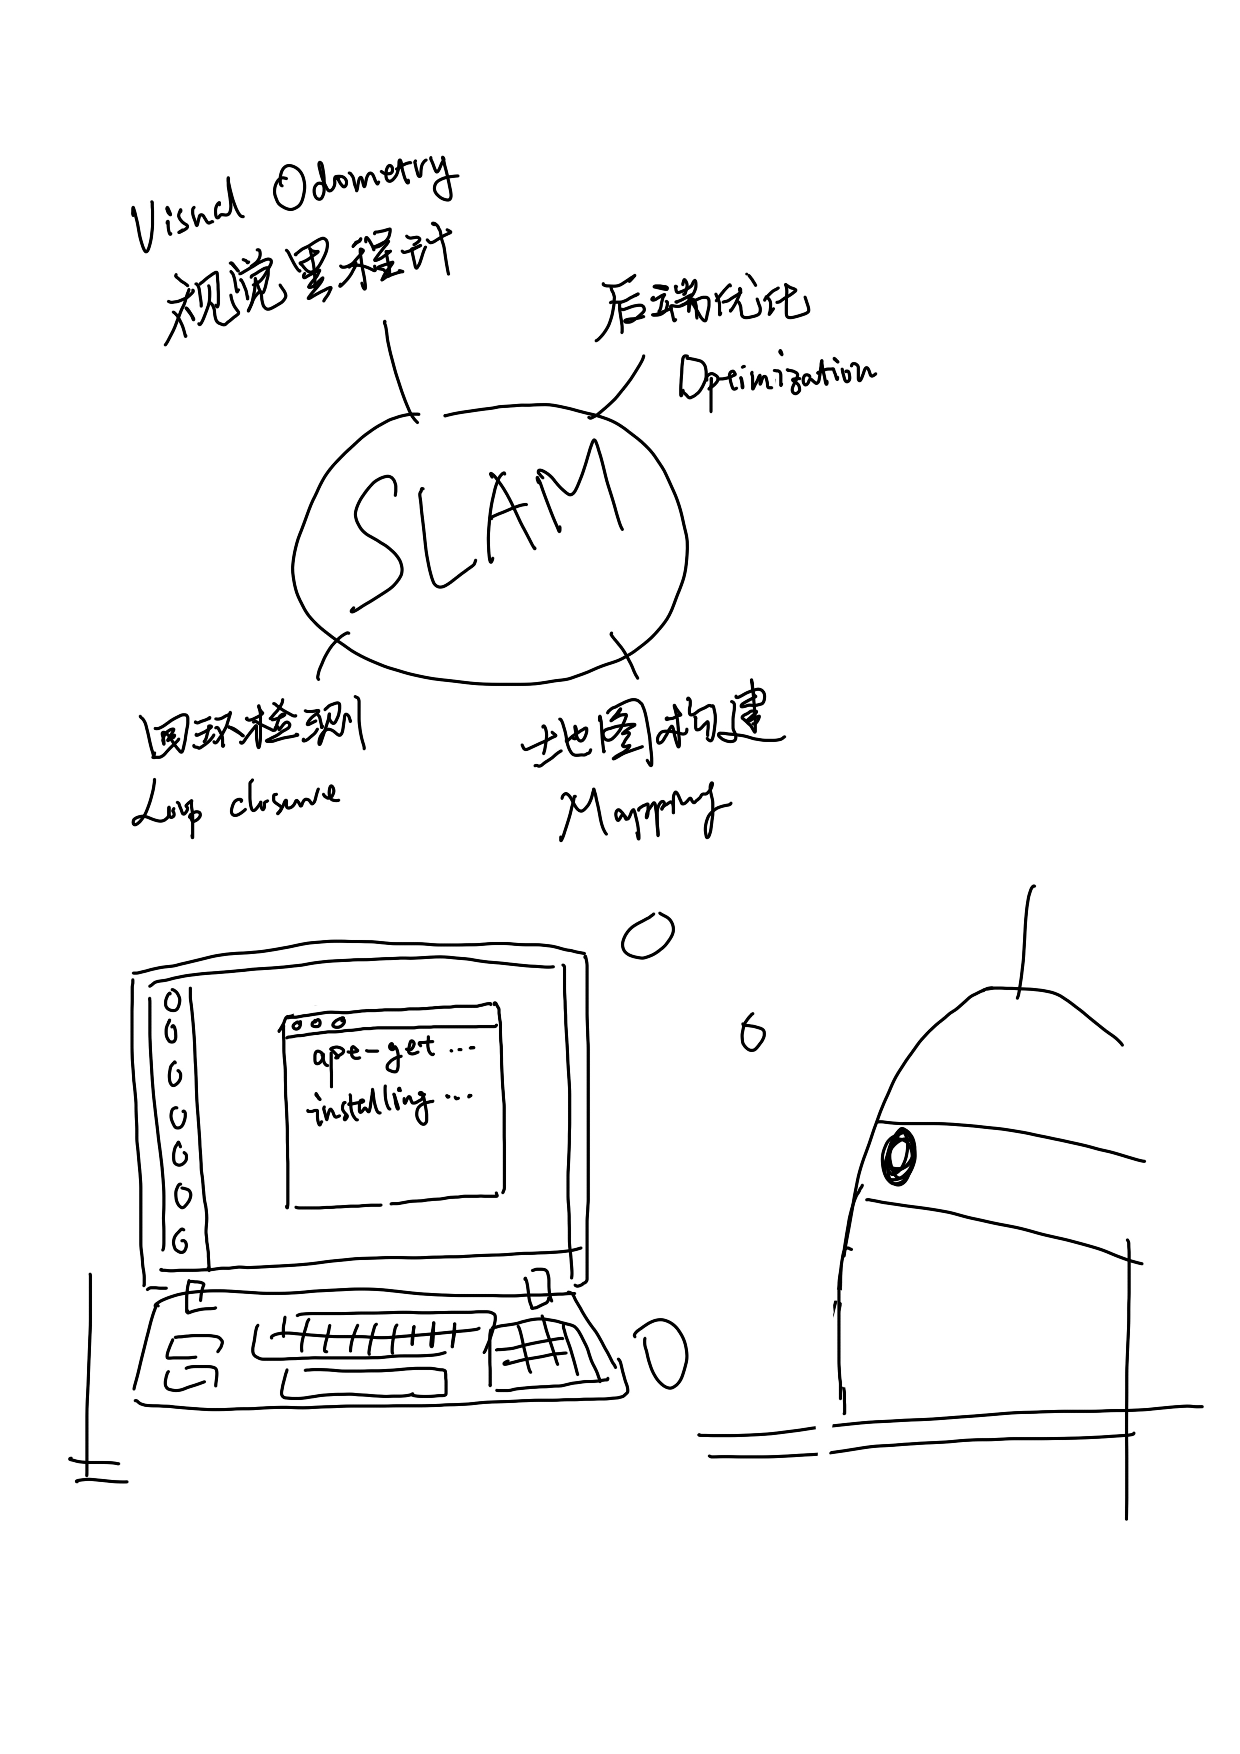
\includepdf{resources/other/ch2.pdf}

\newpage

\section{引子:小萝卜的例子}
% 我发现上来就给出一列符号,讲“SLAM的数学定义”这样的方式,会让初学者觉得难以接受。从一个实际的例子谈起会更好一些。
假设我们组装了一台叫作“小萝卜”的机器人,大概的样子如\autoref{fig:carrot}所示。%(由于工程制图要求严格一些,所以这张图就不手绘了。)

\begin{figure}[!ht]
	\centering
	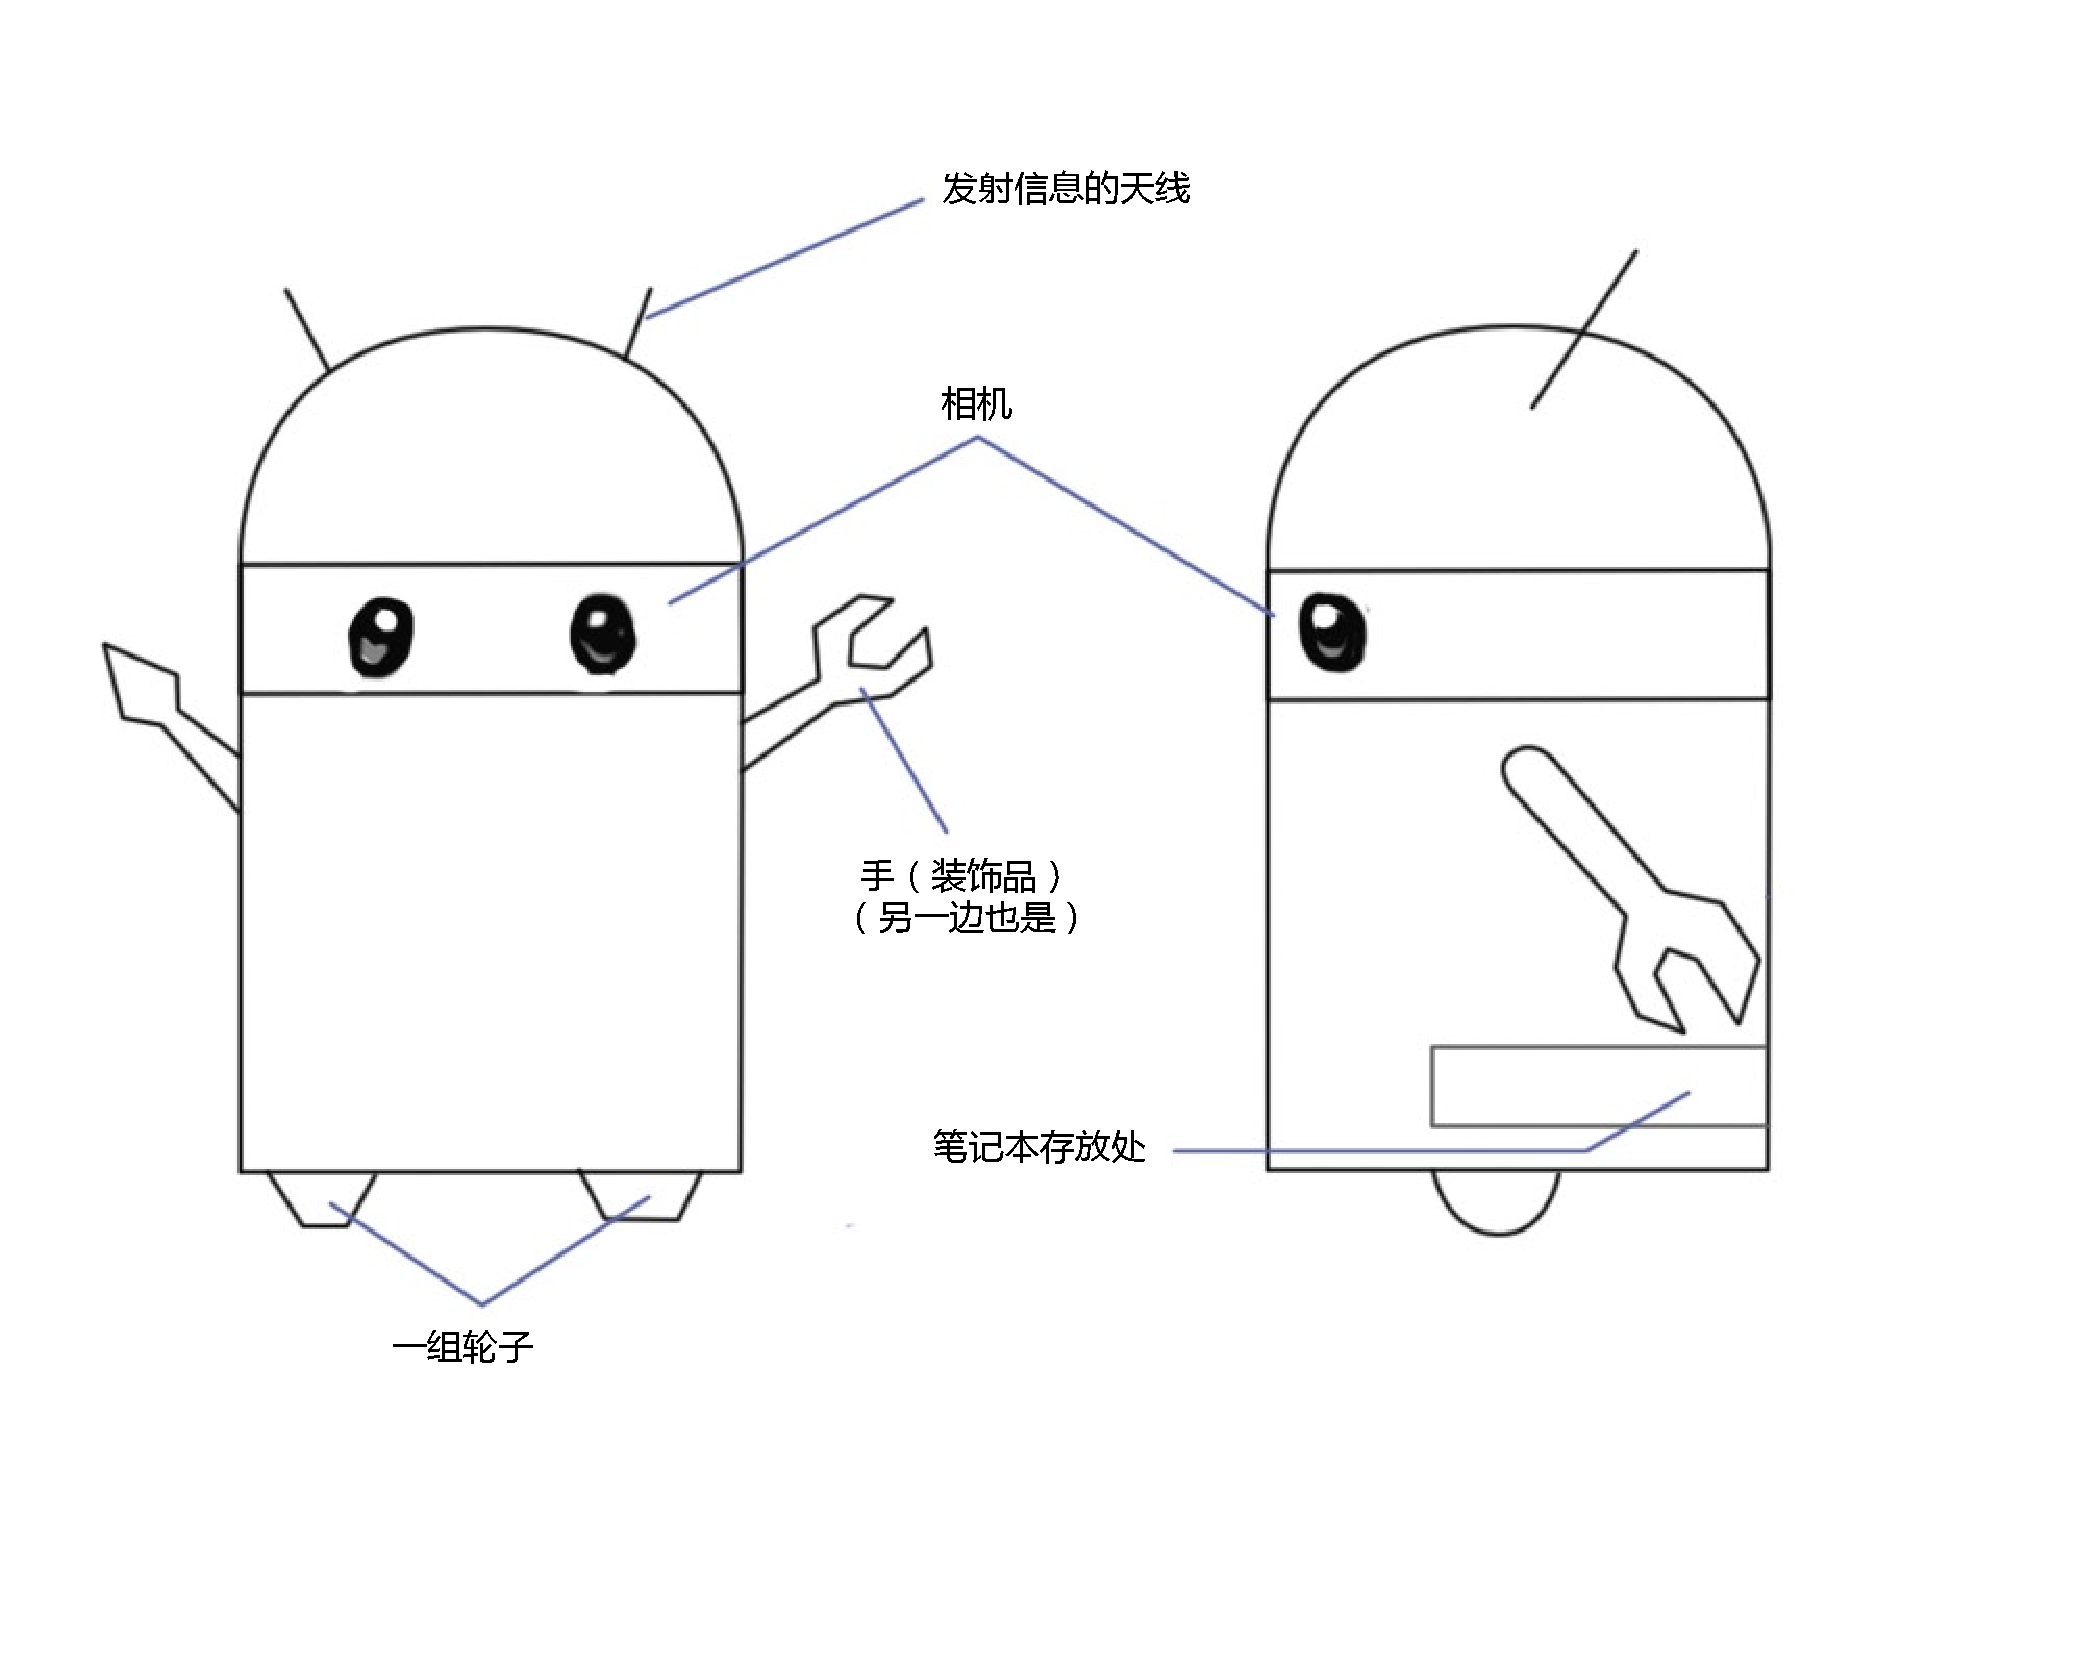
\includegraphics[width=0.7\textwidth]{whatIsSLAM/carrot.pdf}
	\caption{小萝卜设计图。左边:正视图;右边:侧视图。设备有相机、轮子、笔记本,手是装饰品。}
	\label{fig:carrot}
\end{figure}

虽然有点像“安卓”,但它并不是靠安卓系统来计算的。我们把一台笔记本塞进了它的后备箱内(方便我们随时拿出来调试程序)。它能做点什么呢?

我们希望小萝卜具有\textbf{自主运动能力}。虽然世界上也有放在桌面像摆件一样的机器人,能够和人说话或播放音乐,不过一台平板电脑完全可以胜任这些事情。作为机器人,我们希望小萝卜能够在房间里自由移动。不管我们在哪里招呼一声,它都会滴溜溜地走过来。

要移动首先得有轮子和电机,所以我们在小萝卜的下方安装了轮子(足式机器人步态很复杂,我们暂时不考虑)。有了轮子,机器人就能够四处行动了,但不加控制的话,小萝卜不知道行动的目标,就只能四处乱走,更糟糕的情况下会撞上墙造成损毁。为了避免这种情况的发生,我们在它的脑袋上安装了一个相机。安装相机的主要动机,是考虑到这样一个机器人\textbf{和人类非常相似}——从画面上一眼就能看出。有眼睛、大脑和四肢的人类,能够在任意环境里轻松自在地行走、探索,我们(天真地)觉得机器人也能够完成这件事。为了使小萝卜能够探索一个房间,它至少需要知道两件事:

\begin{enumerate}
	\item 我在什么地方?——定位。
	\item 周围环境是什么样?——建图。
\end{enumerate}

“定位”和“建图”,可以看成感知的“内外之分”。作为一个“内外兼修”的小萝卜,一方面要明白自身的\textbf{状态}(即位置),另一方面也要了解外在的\textbf{环境}(即地图)。当然,解决这两个问题的方法非常多。比方说,我们可以在房间地板上铺设导引线,在墙壁上贴识别二维码,在桌子上放置无线电定位设备。如果在室外,还可以在小萝卜脑袋上安装定位设备(像手机或汽车一样)。有了这些东西之后,定位问题是否已经解决了呢?我们不妨把这些传感器(见\autoref{fig:sensors})分为两类。

一类传感器是\textbf{携带于机器人本体上}的,例如机器人的轮式编码器、相机、激光传感器,等等。另一类是\textbf{安装于环境中}的,例如前面讲的导轨、二维码标志,等等。安装于环境中的传感设备,通常能够直接测量到机器人的位置信息,简单有效地解决定位问题。然而,由于它们必须在环境中设置,在一定程度上限制了机器人的使用范围。比方说,有些地方没有GPS信号,有些地方无法铺设导轨,这时该怎么做定位呢?

\begin{figure}[!ht]
	\centering
	\includegraphics[width=1.0\textwidth]{whatIsSLAM/sensors.pdf}
	\caption{一些传感器。(a)利用二维码进行定位的增强现实软件;(b)GPS定位装置;(c)铺设导轨的小车;(d)激光雷达;(e)IMU单元;(f)双目相机。}
	\label{fig:sensors}
\end{figure}

我们看到,这类传感器\textbf{约束}了外部环境。只有在这些约束满足时,基于它们的定位方案才能工作。反之,当约束无法满足时,我们就没法进行定位了。所以说,虽然这类传感器简单可靠,但它们无法提供一个普遍的、通用的解决方案。相对地,那些携带于机器人本体上的传感器,比如激光传感器、相机、轮式编码器、惯性测量单元(Inertial Measurement Unit,IMU)等,它们测到的通常都是一些间接的物理量而不是直接的位置数据。例如,轮式编码器会测到轮子转动的角度,IMU测量运动的角速度和加速度,相机和激光传感器则读取外部环境的某种观测数据。我们只能通过一些间接的手段,从这些数据推算自己的位置。虽然这听上去是一种迂回战术,但更明显的好处是,它没有对环境提出任何要求,从而使得这种定位方案可适用于未知环境。

\clearpage
回顾前面讨论过的SLAM定义,我们在SLAM中非常强调未知环境。在理论上,我们没法限制小萝卜的使用环境\footnote{不过现实中我们都会有一个大概的范围,例如室内和室外的区分。},这意味着我们没法假设像GPS这些外部传感器都能顺利工作。因此,使用携带式的传感器来完成SLAM是我们重点关心的问题。特别地,当谈论视觉SLAM时,我们主要是指如何用\textbf{相机}解决定位和建图问题。

视觉SLAM是本书的主题,所以我们尤其关心小萝卜的眼睛能够做些什么事。SLAM中使用的相机与我们平时见到的单反摄像头并不是同一个东西。它往往更加简单,不携带昂贵的镜头,而是以一定速率拍摄周围的环境,形成一个连续的视频流。普通的摄像头能以每秒钟30张图片的速度采集图像,高速相机则更快一些。按照工作方式的不同,相机可以分为单目相机(Monocular)、双目相机(Stereo)和深度相机(RGB-D)三大类,如\autoref{fig:camera}所示。直观看来,单目相机只有一个摄像头,双目有两个,而RGB-D原理较复杂,除了能够采集到彩色图片之外,还能读出每个像素与相机之间的距离。深度相机通常携带多个摄像头,工作原理和普通相机不尽相同,在第5讲会详细介绍其工作原理,此处读者只需有一个直观概念即可。此外,SLAM中还有全景相机\textsuperscript{\cite{Pretto2011}}、Event相机\textsuperscript{\cite{Rueckauer2016}}等特殊或新兴的种类。虽然偶尔能看到它们在SLAM中的应用,不过到目前为止还没有成为主流。从样子上看,小萝卜使用的似乎是双目相机\footnote{画成单目会比较吓人。}。

\begin{figure}[!ht]
	\centering
	\includegraphics[width=0.8\textwidth]{whatIsSLAM/camera.pdf}
	\caption{形形色色的相机:单目、双目和深度相机。}
	\label{fig:camera}
\end{figure}

我们来分别看一看各种相机用来做SLAM时有什么特点。

\subsubsection{单目相机}
只使用一个摄像头进行SLAM的做法称为单目SLAM(Monocular SLAM)。这种传感器结构特别简单,成本特别低,所以单目SLAM非常受研究者关注。你肯定见过单目相机的数据:照片。是的,作为一张照片,它有什么特点呢?

照片本质上是拍照时的场景(Scene)在相机的成像平面上留下的一个\textbf{投影}。\textbf{它以二维的形式反映了三维的世界。}显然,这个过程丢掉了场景的一个维度,也就是所谓的深度(或距离)。在单目相机中,我们无法通过单张图片来计算场景中物体与我们之间的\textbf{距离}(远近)。之后我们会看到,这个距离将是SLAM中非常关键的信息。由于我们人类见过大量的图像,形成了一种天生的直觉,对大部分场景都有一个直观的\textbf{距离感(空间感)},它可以帮助我们判断图像中物体的远近关系。比如说,我们能够辨认出图像中的物体,并且知道其大致的大小;比如,近处的物体会挡住远处的物体,而太阳、月亮等天体一般在很远的地方;再如,物体受光照后会留下影子,等等。这些信息都可以帮助我们判断物体的远近,但也存在一些情况会使这种距离感失效,这时我们就无法判断物体的远近及其真实大小了。\autoref{fig:why-depth}~所示就是这样一个例子。在这张图像中,我们无法仅通过它来判断后面那些小人是真实的人,还是小型模型。除非我们转换视角,观察场景的三维结构。换言之,在单张图像里,你无法确定一个物体的真实大小。它可能是一个很大但很远的物体,也可能是一个很近但很小的物体。由于近大远小的原因,它们可能在图像中变成同样大小的样子。

\begin{figure}[!htp]
	\centering
	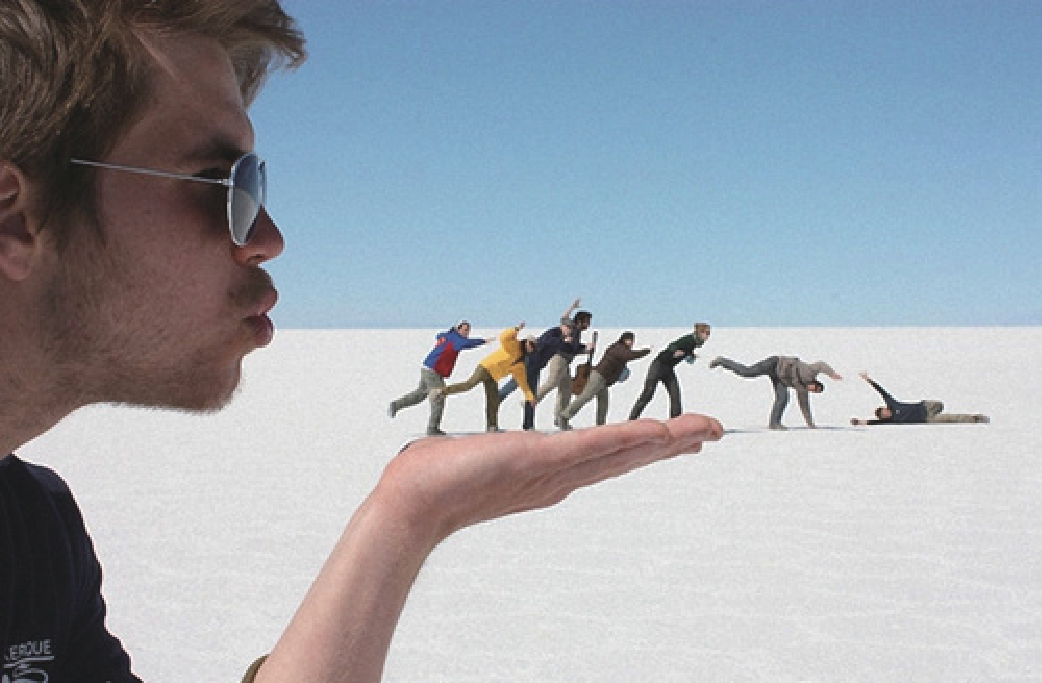
\includegraphics[width=0.7\textwidth]{whatIsSLAM/why-depth.pdf}
	\caption{单目视觉中的尴尬:不知道深度时,手掌上的人是真人还是模型?}
	\label{fig:why-depth}
\end{figure}

由于单目相机拍摄的图像只是三维空间的二维投影,所以,如果真想恢复三维结构,必须改变相机的视角。在单目SLAM中也是同样的原理。我们必须移动相机,才能估计它的\textbf{运动}(Motion),同时估计场景中物体的远近和大小,不妨称之为\textbf{结构}(Structure)。那么,怎么估计这些运动和结构呢?从生活经验中我们知道,如果相机往右移动,那么图像里的东西就会往左边移动——这就给我们推测运动带来了信息。另一方面,我们还知道:\textbf{近处的物体移动快,远处的物体则运动缓慢}。于是,当相机移动时,这些物体在图像上的运动就形成了\textbf{视差}。通过视差,我们就能定量地判断哪些物体离得远,哪些物体离得近。

然而,即使我们知道了物体远近,它们仍然只是一个相对的值。比如我们在看电影时,虽然能够知道电影场景中哪些物体比另一些大,但无法确定电影里那些物体的“真实尺度”:那些大楼是真实的高楼大厦,还是放在桌上的模型?而摧毁大厦的是真实怪兽,还是穿着特摄服装的演员?直观地说,如果把相机的运动和场景大小同时放大两倍,单目相机所看到的像是一样的。同样地,把这个大小乘以任意倍数,我们都将看到一样的景象。这说明,单目SLAM估计的轨迹和地图将与真实的轨迹和地图相差一个因子,也就是所谓的\textbf{尺度}(Scale)\footnote{数学上的原因将会在视觉里程计一讲中解释。}。由于单目SLAM无法仅凭图像确定这个真实尺度,所以又称为\textbf{尺度不确定性}。

平移之后才能计算深度,以及无法确定真实尺度,这两件事情给单目SLAM的应用造成了很大的麻烦。其根本原因是通过单张图像无法确定深度。所以,为了得到这个深度,人们开始使用双目和深度相机。

\subsubsection{双目相机和深度相机}

使用双目相机和深度相机的目的,在于通过某种手段测量物体与我们之间的距离,克服单目相机无法知道距离的缺点。一旦知道了距离,场景的三维结构就可以通过单个图像恢复出来,也就消除了尺度不确定性。尽管都是为了测量距离,但双目相机与深度相机测量深度的原理是不一样的。双目相机由两个单目相机组成,但这两个相机之间的距离﹝称为\textbf{基线}(Baseline)﹞是已知的。我们通过这个基线来估计每个像素的空间位置——这和人眼非常相似。我们人类可以通过左右眼图像的差异判断物体的远近,在计算机上也是同样的道理(见\autoref{fig:stereo})。如果对双目相机进行拓展,也可以搭建多目相机,不过本质上并没有什么不同。

\begin{figure}[!ht]
	\centering
	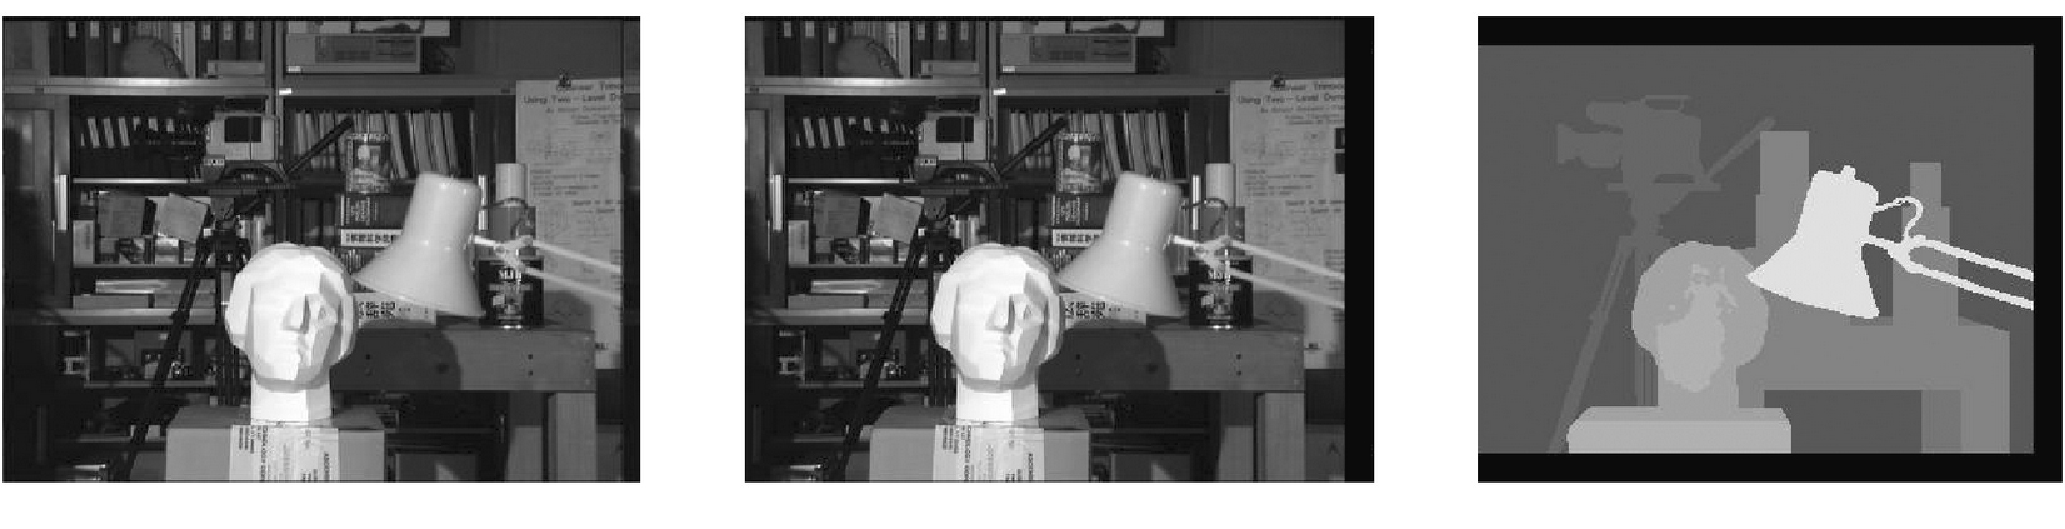
\includegraphics[width=1.0\textwidth]{whatIsSLAM/stereo.pdf}
	\caption{双目相机的数据:左眼图像,右眼图像。通过左右眼的差异,能够判断场景中物体与相机之间的距离。}
	\label{fig:stereo}
\end{figure}

计算机上的双目相机需要大量的计算才能(不太可靠地)估计每一个像素点的深度,相比于人类真是非常笨拙。双目相机测量到的深度范围与基线相关。基线距离越大,能够测量到的就越远,所以无人车上搭载的双目通常会是个很大的家伙。双目相机的距离估计是比较左右眼的图像获得的,并不依赖其他传感设备,所以它既可以应用在室内,亦可应用于室外。双目或多目相机的缺点是配置与标定均较为复杂,其深度量程和精度受双目的基线与分辨率所限,而且视差的计算非常消耗计算资源,需要使用GPU和FPGA设备加速后,才能实时输出整张图像的距离信息。因此在现有的条件下,计算量是双目的主要问题之一。

深度相机(又称RGB-D相机,在本书中主要使用RGB-D这个名称)是2010年左右开始兴起的一种相机,它最大的特点是可以通过红外结构光或Time-of-Flight(ToF)原理,像激光传感器那样,通过主动向物体发射光并接收返回的光,测出物体与相机之间的距离。这部分并不像双目相机那样通过软件计算来解决,而是通过物理的测量手段,所以相比于双目相机可节省大量的计算(见\autoref{fig:rgbd})。目前常用的RGB-D相机包括Kinect/Kinect V2、Xtion Pro Live、RealSense等。不过,现在多数RGB-D相机还存在测量范围窄、噪声大、视野小、易受日光干扰、无法测量透射材质等诸多问题,在SLAM方面,主要用于室内,室外则较难应用。

\begin{figure}[!ht]
	\centering
	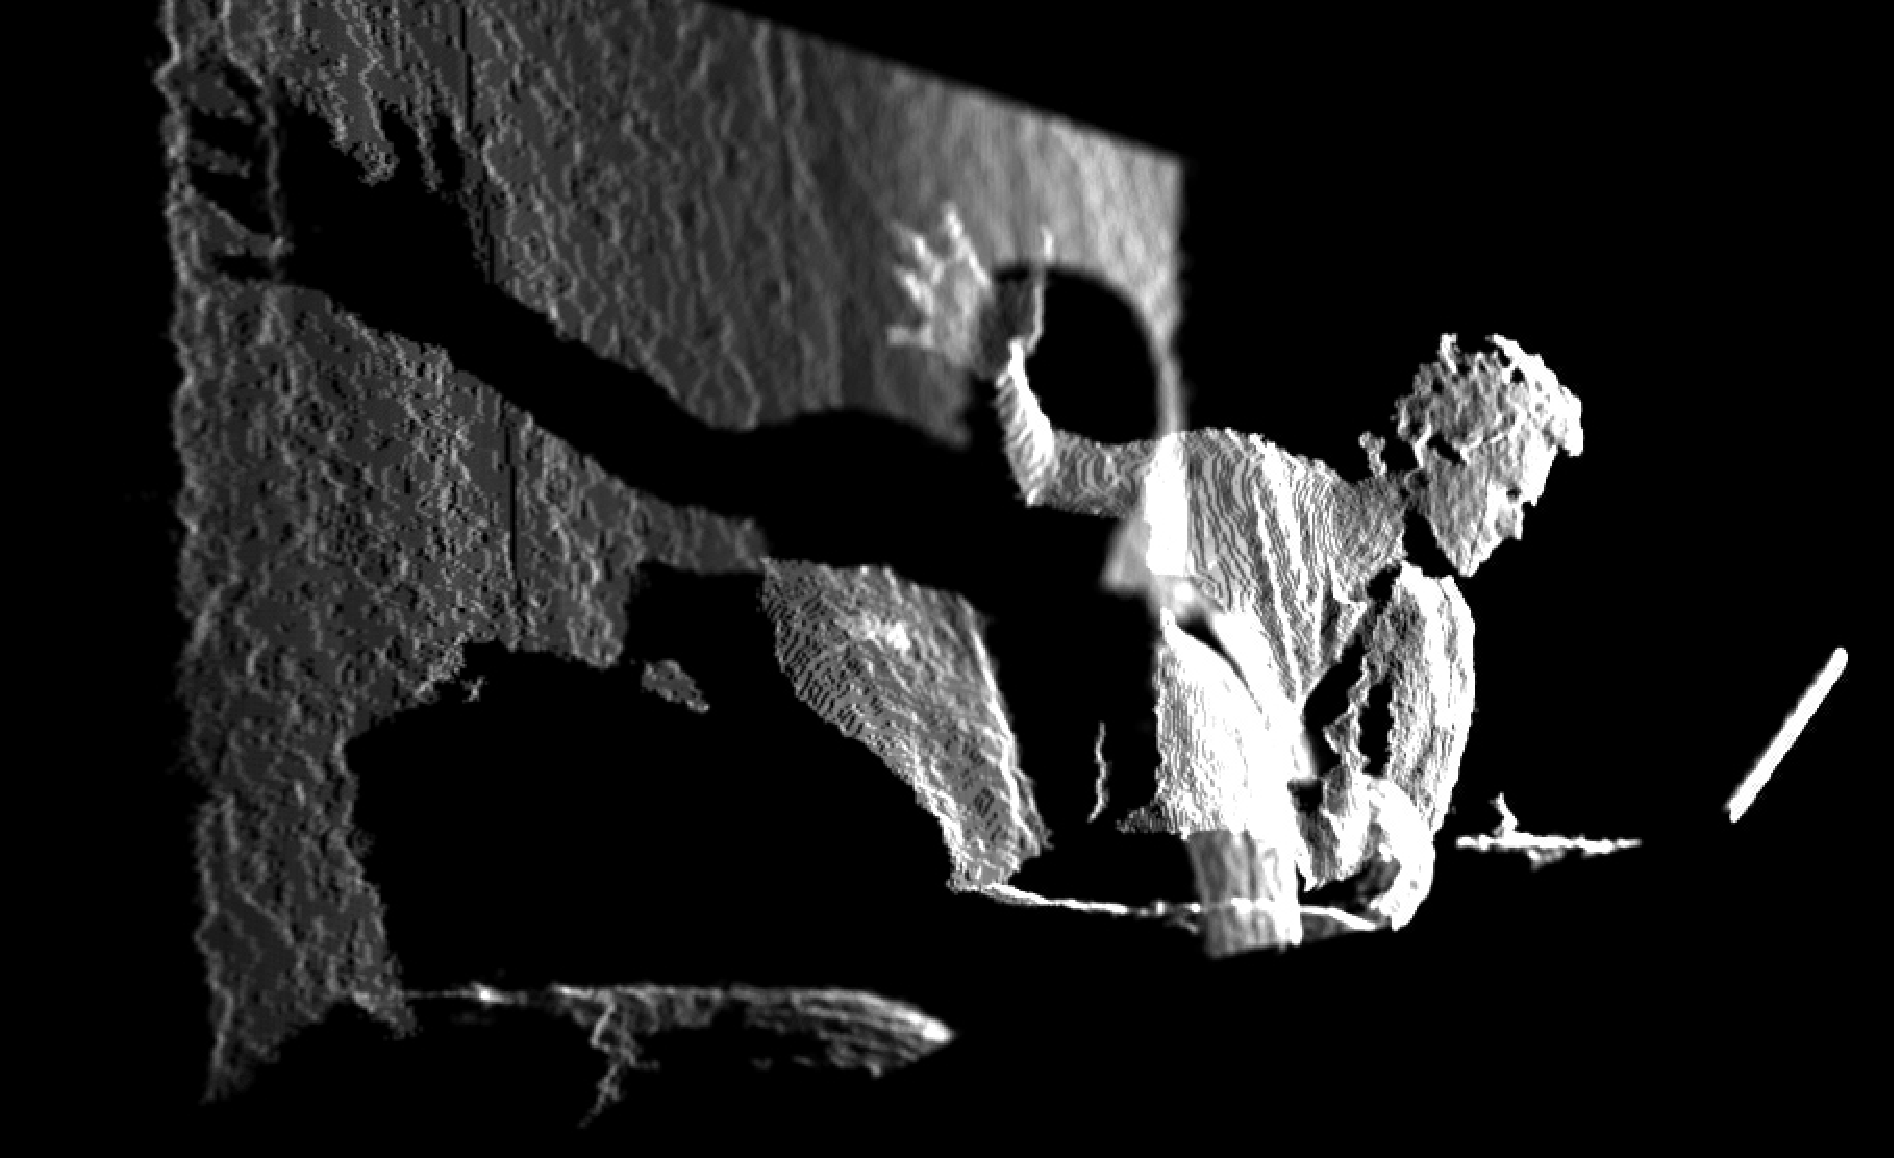
\includegraphics[width=0.8\textwidth]{whatIsSLAM/rgbd.pdf}
	\caption{RGB-D数据:深度相机可以直接测量物体的图像和距离,从而恢复三维结构。}
	\label{fig:rgbd}
\end{figure}

我们讨论了几种常见的相机,相信通过以上的说明,你已经对它们有了直观的了解。现在,想象相机在场景中运动的过程,我们将得到一系列连续变化的图像\footnote{你可以用手机录个小视频试试。}。视觉SLAM的目标,是通过这样的一些图像,进行定位和地图构建。这件事情并没有我们想象的那么简单。它不是某种算法,只要我们输入数据,就可以往外不断地输出定位和地图信息了。SLAM需要一个完善的算法框架,而经过研究者们长期的努力工作,现有这个框架已经定型了。

\section{经典视觉SLAM框架}
下面来看经典的视觉SLAM框架,如\autoref{fig:overflow}所示,了解一下视觉SLAM究竟由哪几个模块组成。

\begin{figure}[!htp]
	\centering
	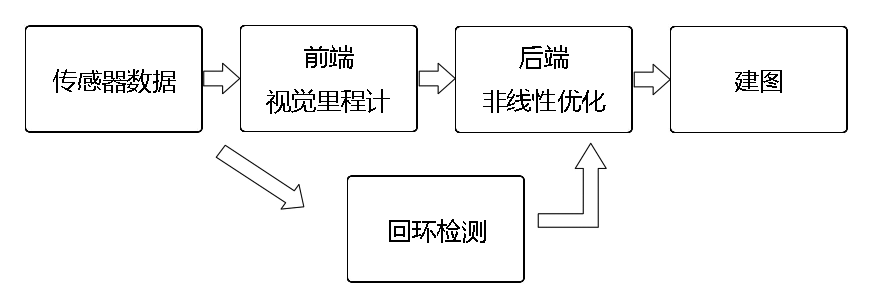
\includegraphics[width=0.8\textwidth]{whatIsSLAM/overflow.pdf}
	\caption{整体视觉SLAM流程图。}
	\label{fig:overflow}
\end{figure}

整个视觉SLAM流程包括以下步骤。
\begin{enumerate}
	\item 传感器信息读取。在视觉SLAM中主要为相机图像信息的读取和预处理。如果是在机器人中,还可能有码盘、惯性传感器等信息的读取和同步。
	\item \textbf{视觉里程计}(Visual Odometry,VO)。视觉里程计的任务是估算相邻图像间相机的运动,以及局部地图的样子。VO又称为前端(Front End)。
	\item \textbf{后端优化}(Optimization)。后端接受不同时刻视觉里程计测量的相机位姿,以及回环检测的信息,对它们进行优化,得到全局一致的轨迹和地图。由于接在VO之后,又称为后端(Back End)。
	\item \textbf{回环检测}(Loop Closing)。回环检测判断机器人是否到达过先前的位置。如果检测到回环,它会把信息提供给后端进行处理。
	\item \textbf{建图}(Mapping)。它根据估计的轨迹,建立与任务要求对应的地图。
\end{enumerate}

经典的视觉SLAM框架是过去十几年的研究成果。这个框架本身及其所包含的算法已经基本定型,并且已经在许多视觉程序库和机器人程序库中提供。依靠这些算法,我们能够构建一个视觉SLAM系统,使之在正常的工作环境里实时定位与建图。因此,我们说,\textbf{如果把工作环境限定在静态、刚体,光照变化不明显、没有人为干扰的场景},那么,这个SLAM系统是相当成熟的了\textsuperscript{\cite{Cadena2016}}。

读者可能还没有理解上面几个模块的概念,下面就来详细介绍各个模块具体的任务。但是,准确理解其工作原理需要一些数学知识,我们将放到本书的第二部分进行。这里读者只需对各模块有一个直观的、定性的理解即可。

\subsection{视觉里程计}
视觉里程计关心的是\textbf{相邻图像}之间的相机运动,最简单的情况当然是两张图像之间的运动关系。例如,当看到\autoref{fig:cameramotion}时,我们会自然地反应出右图应该是左图向左旋转一定角度的结果(在视频情况下感觉会更加自然)。我们不妨思考一下:自己是怎么知道“向左旋转”这件事情的呢?人类早已习惯于用眼睛探索世界,估计自己的位置,但又往往难以用理性的语言描述我们的直觉。看到\autoref{fig:cameramotion}时,我们会自然地认为,这个场景中离我们近的是吧台,远处是墙壁和黑板。当相机向左转动时,吧台离我们近的部分出现在视野中,而右侧远处的柜子则移出了视野。通过这些信息,我们判断相机应该是向左旋转了。

\begin{figure}[!ht]
	\centering
	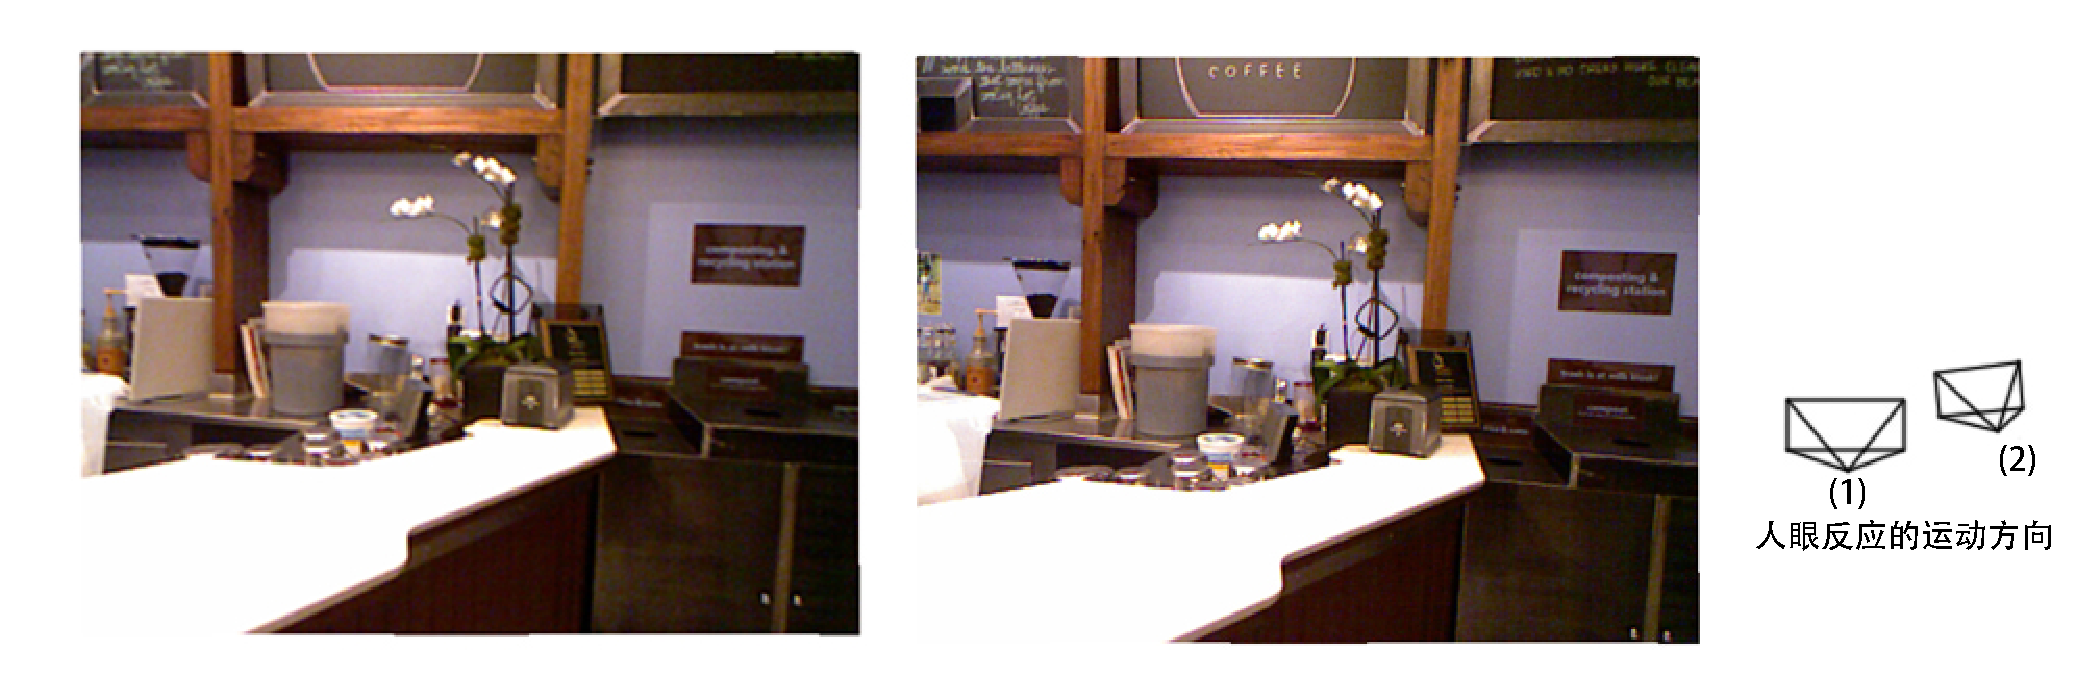
\includegraphics[width=0.8\textwidth]{whatIsSLAM/cameramotion.pdf}
	\caption{相机拍摄到的图片与人眼反应的运动方向。}
	\label{fig:cameramotion}
\end{figure}

但是,如果进一步问:能否确定旋转了多少度,平移了多少厘米?我们就很难给出一个确切的答案了。因为我们的直觉对这些具体的数字并不敏感。但是,在计算机中,又必须精确地测量这段运动信息。所以我们要问:\textbf{计算机是如何通过图像确定相机的运动的呢?}

前面也提过,在计算机视觉领域,人类在直觉上看来十分自然的事情,在计算机视觉中却非常困难。图像在计算机里只是一个数值矩阵。这个矩阵里表达着什么东西,计算机毫无概念(这也正是现在机器学习要解决的问题)。而在视觉SLAM中,我们只能看到一个个像素,知道它们是某些空间点在相机的成像平面上投影的结果。所以,为了定量地估计相机运动,必须先\textbf{了解相机与空间点的几何关系}。

要讲清这个几何关系以及VO的实现方法,需要铺垫一些背景知识。在这里我们先让读者对VO有个直观的概念。现在只需知道,VO能够通过相邻帧间的图像估计相机运动,并恢复场景的空间结构。称它为“里程计”是因为它和实际的里程计一样,只计算相邻时刻的运动,而和再往前的过去的信息没有关联。在这一点上,VO就像一种只有短时间记忆的物种。

现在,假定我们已有了一个视觉里程计,估计了两张图像间的相机运动。那么,只要把相邻时刻的运动“串”起来,就构成了机器人的运动轨迹,从而解决了定位问题。另一方面,我们根据每个时刻的相机位置,计算出各像素对应的空间点的位置,就得到了地图。这么说来,有了VO,是不是就解决了SLAM问题呢?

视觉里程计确实是SLAM的关键,我们也会花大量的篇幅来介绍它。然而,仅通过视觉里程计来估计轨迹,将不可避免地出现\textbf{累积漂移}(Accumulating Drift)。这是由于视觉里程计(在最简单的情况下)只估计两个图像间的运动造成的。我们知道,每次估计都带有一定的误差,而由于里程计的工作方式,先前时刻的误差将会传递到下一时刻,导致经过一段时间之后,估计的轨迹将不再准确(见\autoref{fig:loopclosure})。比方说,机器人先向左转$90^\circ$,再向右转$90^\circ$。由于误差,我们把第一个$90^\circ$估计成了$89^\circ$。那我们就会尴尬地发现,向右转之后机器人的估计位置并没有回到原点。更糟糕的是,即使之后的估计再准确,与真实值相比,都会带上这$-1^\circ$的误差。

\begin{figure}[!htp]
	\centering
	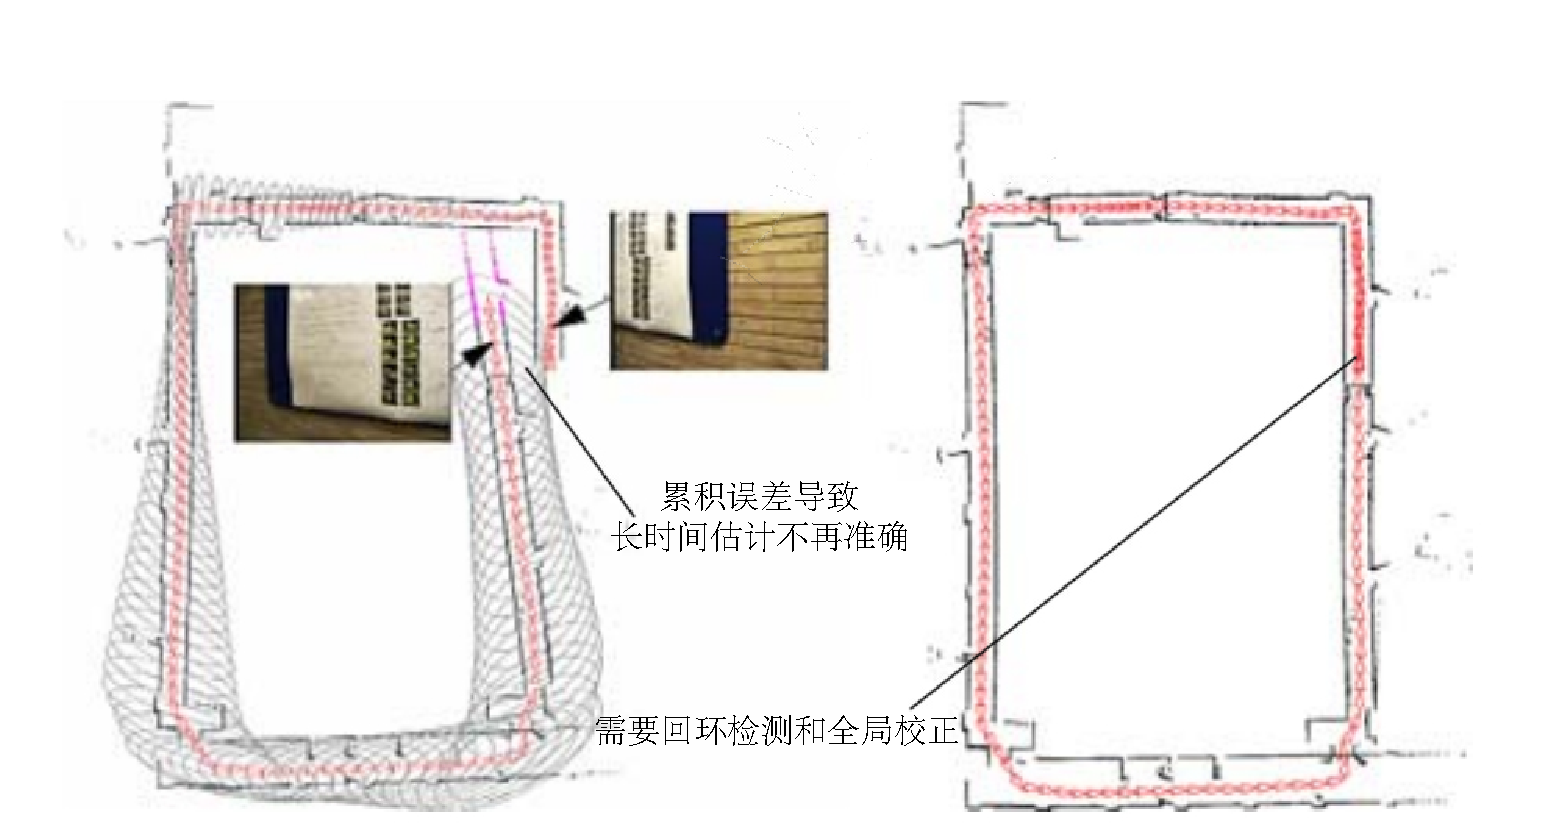
\includegraphics[width=0.8\textwidth]{whatIsSLAM/loopclosure.pdf}
	\caption{累积误差与回环检测的校正结果\textsuperscript{\cite{Newman2005}}。}
	\label{fig:loopclosure}
\end{figure}

这也就是所谓的\textbf{漂移}(Drift)。它将导致我们无法建立一致的地图。你会发现原本直的走廊变成了斜的,而原本$90^\circ$的直角变成了歪的——这实在是一件令人难以忍受的事情!为了解决漂移问题,我们还需要两种技术:\textbf{后端优化}\footnote{更多时候称为后端(Back End)。由于主要使用的是优化方法,故称为后端优化。}和\textbf{回环检测}。回环检测负责把“机器人回到原始位置”的事情检测出来,而后端优化则根据该信息,校正整个轨迹的形状。

\subsection{后端优化}
笼统地说,后端优化主要指处理SLAM过程中\textbf{噪声}的问题。虽然我们很希望所有的数据都是准确的,然而现实中,再精确的传感器也带有一定的噪声。便宜的传感器测量误差较大,昂贵的可能会小一些,有的传感器还会受磁场、温度的影响。所以,除了解决“如何从图像估计出相机运动”之外,我们还要关心这个估计带有多大的噪声,这些噪声是如何从上一时刻传递到下一时刻的,而我们又对当前的估计有多大的自信。后端优化要考虑的问题,就是如何从这些带有噪声的数据中估计整个系统的状态,以及这个状态估计的不确定性有多大——这称为最大后验概率估计(Maximum-a-Posteriori,MAP)。这里的状态既包括机器人自身的轨迹,也包含地图。

相对地,视觉里程计部分有时被称为“前端”。在SLAM框架中,前端给后端提供待优化的数据,以及这些数据的初始值。而后端负责整体的优化过程,它往往面对的只有数据,不必关心这些数据到底来自什么传感器。\textbf{在视觉SLAM中,前端和计算机视觉研究领域更为相关,比如图像的特征提取与匹配等,后端则主要是滤波与非线性优化算法。}

从历史意义上来说,现在我们称为后端优化的部分,很长一段时间直接被称为“SLAM研究”。早期的SLAM问题是一个状态估计问题——正是后端优化要解决的东西。在最早提出SLAM的一系列论文中,当时的人们称它为“空间状态不确定性的估计”(Spatial Uncertainty)\textsuperscript{\cite{Smith1986, Smith1990}}。虽然有一些晦涩,但也确实反映出了SLAM问题的本质:\textbf{对运动主体自身和周围环境空间不确定性的估计}。为了解决SLAM问题,我们需要状态估计理论,把定位和建图的不确定性表达出来,然后采用滤波器或非线性优化,估计状态的均值和不确定性(方差)。状态估计与非线性优化的具体内容将在第6讲、第10讲和第11讲介绍。让我们暂时跳过它的原理说明,继续往下介绍。

\subsection{回环检测}

回环检测,又称闭环检测(Loop Closure Detection),主要解决位置估计\textbf{随时间漂移}的问题。怎么解决呢?假设实际情况下机器人经过一段时间的运动后回到了原点,但是由于漂移,它的位置估计值却没有回到原点。怎么办呢?我们想,如果有某种手段,让机器人知道“回到了原点”这件事,或者把“原点”识别出来,我们再把位置估计值“拉”过去,就可以消除漂移了。这就是所谓的回环检测。

回环检测与“定位”和“建图”二者都有密切的关系。事实上,我们认为,地图存在的主要意义是让机器人知晓自己到过的地方。为了实现回环检测,我们需要让机器人具有\textbf{识别到过的场景}的能力。它的实现手段有很多。例如像前面说的那样,我们可以在机器人下方设置一个标志物(如一张二维码图片)。它只要看到了这个标志,就知道自己回到了原点。但是,该标志物实质上是一种环境中的传感器,对应用环境做了限制(万一不能贴二维码怎么办?)。我们更希望机器人能使用携带的传感器——也就是图像本身,来完成这一任务。例如,可以判断\textbf{图像间的相似性}来完成回环检测。这一点和人是相似的。当我们看到两张相似的图片时,容易辨认它们来自同一个地方。如果回环检测成功,可以显著地减小累积误差。所以,视觉回环检测实质上是一种计算图像数据相似性的算法。由于图像的信息非常丰富,使得正确检测回环的难度降低了不少。

在检测到回环之后,我们会把“A与B是同一个点”这样的信息告诉后端优化算法。然后,后端根据这些新的信息,把轨迹和地图调整到符合回环检测结果的样子。这样,如果我们有充分而且正确的回环检测,就可以消除累积误差,得到全局一致的轨迹和地图。

%对于视觉SLAM,多数系统采用目前较为成熟的词袋模型(Bag-of-Words, BoW)。词袋模型把图像中的视觉特征(SIFT, SURF等)聚类,然后建立词典,进而寻找每个图中含有哪些“单词”(word)。也有研究者使用传统模式识别的方法,把回环检测建构成一个分类问题,训练分类器进行分类。
%
%但是回环检测的困难也是存在的,主要在于\textbf{错误的检测结果可能使地图变得很糟糕}。错误可分为两类:1.假阳性(False Positive),又称感知偏差(Perceptual Aliasing),指事实上不同的场景被当成了同一个。这主要来自一些看似相同的场景,然而实际上是两个不同的地方。这种情况在人工建筑物普遍存在,例如一幢楼里很多门、窗、厕所、走廓,都十分地相似,很容易被当成同一个。2. 假阴性(False Negative),又称感知变异(Perceptual Variability),指实际上同一个场景被当成了两个。在视觉SLAM中,这种情况主要发生在光照变化的场合。例如清晨的阳光洒进窗户,朦胧一片,而正午时分,光线清晰,景物错落可见。虽然人能否通过直觉辨别,但它在计算机图像中的差异如此之大,很难认出这是同一个窗户。
%
%一个好的视觉回环检测算法应该尽量避免出现这两种错误。因此,它要保证两点:
%
%\begin{enumerate}
%	\item 检测出的回环应该是对的。
%	\item 实际发生回环的时候,应该被检测出来。
%\end{enumerate}
%
%前者称为准确率(Perception),后者称为召回率(Recall)。尽管不是必然,但对同一个算法来说,这两者往往是矛盾的:准确率的提升意味着更严格的检测,使得差的回环无法提取出来——从而可能忽略掉真实存在的回环。研究者们常常用准确率-召回率曲线来评价一个回环检测算法的好坏。我们自然希望能够有准确率和召回率都很高的回环检测算法,但现实往往不尽如人意。

% 如果我们有了良好的回环检测和后端优化算法,就能得到一个全局一致性较好的轨迹了。剩下的工作,就是建立一个良好的地图。

\subsection{建图}
建图(Mapping)是指构建地图的过程。地图(见\autoref{fig:map})是对环境的描述,但这个描述并不是固定的,需要视SLAM的应用而定。

\begin{figure}[!htp]
	\centering
	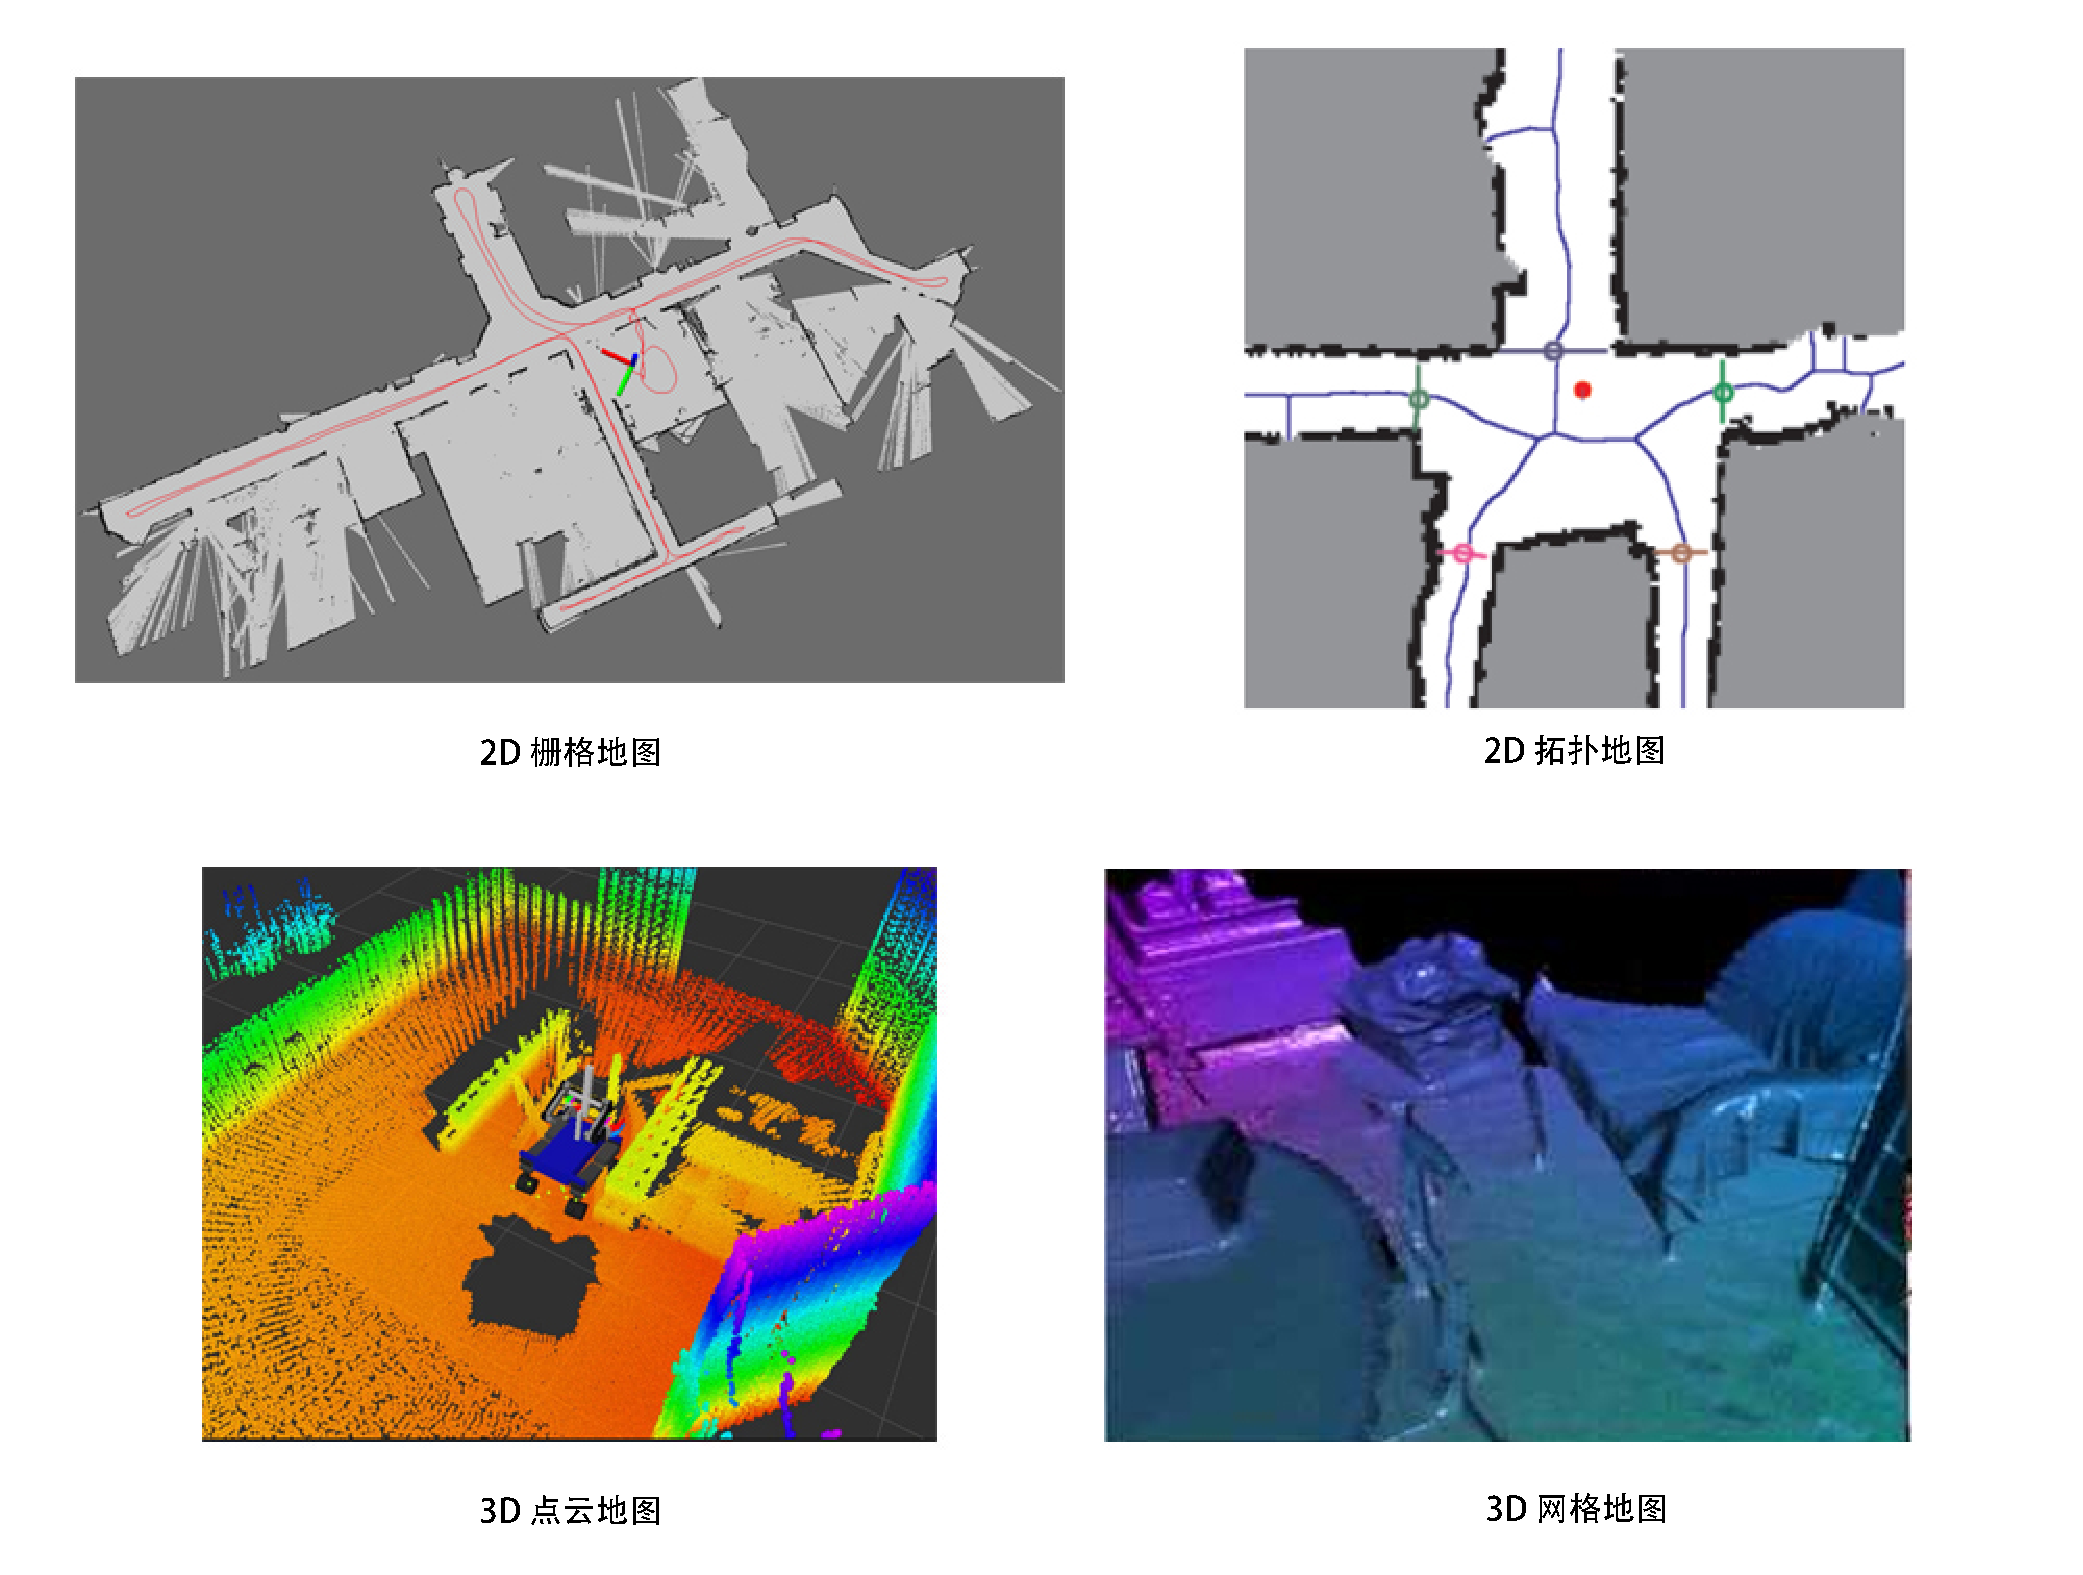
\includegraphics[width=0.8\textwidth]{whatIsSLAM/map.pdf}
	\caption{形形色色的地图\textsuperscript{\cite{Beeson2010}}。}
	\label{fig:map}
\end{figure}

对于家用扫地机器人来说,这种主要在低矮平面里运动的机器人,只需要一个二维的地图,标记哪里可以通过,哪里存在障碍物,就够它在一定范围内导航了。而对于一个相机,它有6自由度的运动,我们至少需要一张三维的地图。有些时候,我们想要一个漂亮的重建结果,不仅是一组空间点,还需要带纹理的三角面片。另一些时候,我们又不关心地图的样子,只需要知道“A点到B点可通过,而B点到C点不行”这样的事情。甚至,有时不需要地图,或者地图可以由其他人提供,例如,行驶的车辆往往可以得到已绘制好的当地地图。

对于地图,我们有太多的想法和需求。因此,相比于前面提到的视觉里程计、回环检测和后端优化,建图并没有一个固定的形式和算法。一组空间点的集合也可以称为地图,一个漂亮的3D模型亦是地图,一个标记着城市、村庄、铁路、河道的图片还是地图。地图的形式随SLAM的应用场合而定。大体上讲,可以分为\textbf{度量地图}与\textbf{拓扑地图}两种。

\clearpage

\subsubsection{度量地图(Metric Map)}
度量地图强调精确地表示地图中物体的位置关系,通常用稀疏(Sparse)与稠密(Dense)对其分类。稀疏地图进行了一定程度的抽象,并不需要表达所有的物体。例如,我们选择一部分具有代表意义的东西,称之为路标(Landmark),那么一张稀疏地图就是由路标组成的地图,而不是路标的部分就可以忽略掉。相对地,稠密地图着重于建模所有看到的东西。对于定位来说,稀疏路标地图就足够了。而用于导航时,则往往需要稠密的地图(否则撞上两个路标之间的墙怎么办?)。稠密地图通常按照某种分辨率,由许多个小块组成。对于二维度量地图是许多个小格子(Grid),而对于三维度量地图则是许多小方块(Voxel)。一般地,一个小块含有占据、空闲、未知三种状态,以表达该格内是否有物体。当查询某个空间位置时,地图能够给出该位置是否可以通过的信息。这样的地图可以用于各种导航算法,如A*、D*\footnote{\url{https://en.wikipedia.org/wiki/A*_search_algorithm}}等,为机器人研究者所重视。但是我们也看到,这种地图需要存储每一个格点的状态,会耗费大量的存储空间,而且多数情况下地图的许多细节部分是无用的。另一方面,大规模度量地图有时会出现一致性问题。很小的一点转向误差,可能会导致两间屋子的墙出现重叠,使地图失效。

\subsubsection{拓扑地图(Topological Map)}
相比于度量地图的精确性,拓扑地图则更强调地图元素之间的关系。拓扑地图是一个图(Graph),由节点和边组成,只考虑节点间的连通性,例如A、B点是连通的,而不考虑如何从A点到达B点。它放松了地图对精确位置的需要,去掉了地图的细节问题,是一种更为紧凑的表达方式。然而,拓扑地图不擅长表达具有复杂结构的地图。如何对地图进行分割形成结点与边,又如何使用拓扑地图进行导航与路径规划,仍是有待研究的问题。

\section{SLAM问题的数学表述}

通过前面的介绍,读者应该对SLAM中各个模块的组成和主要功能有了直观的了解。但仅仅靠直观印象并不能帮助我们写出可以运行的程序。我们要把它上升到理性层次,也就是用数学语言来描述SLAM过程。我们会用到一些变量和公式,但请读者放心,我们会尽量让它保持足够地清楚。

假设小萝卜正携带着某种传感器在未知环境里运动,怎么用数学语言描述这件事呢?首先,由于相机通常是在某些时刻采集数据的,所以我们也只关心这些时刻的位置和地图。这就把一段连续时间的运动变成了离散时刻$t=1, \cdots, K$当中发生的事情。在这些时刻,用$\bm{x}$表示小萝卜自身的位置。于是各时刻的位置就记为$ \bm{x}_1, \cdots, \bm{x}_K$,它们构成了小萝卜的轨迹。地图方面,我们假设地图是由许多个\textbf{路标}(Landmark)组成的,而每个时刻,传感器会测量到一部分路标点,得到它们的观测数据。不妨设路标点一共有$N$个,用$\bm{y}_1, \cdots, \bm{y}_N$表示它们。

在这样的设定中,“小萝卜携带着传感器在环境中运动”,由如下两件事情描述:

\begin{enumerate}
	\item 什么是\textbf{运动}?我们要考虑从$k-1$时刻到$k$时刻,小萝卜的位置$\bm{x}$是如何变化的。
	\item 什么是\textbf{观测}?假设小萝卜在$k$时刻于$\bm{x}_k$处探测到了某一个路标$\bm{y}_j$,我们要考虑这件事情是如何用数学语言来描述的。
\end{enumerate}

先来看运动。通常,机器人会携带一个测量自身运动的传感器,比如说码盘或惯性传感器。这个传感器可以测量有关运动的读数,但不一定直接就是位置之差,还可能是加速度、角速度等信息。然而,无论是什么传感器,我们都能使用一个通用的、抽象的数学模型:
\begin{equation}	
{\bm{x}_k} = f\left( {{\bm{x}_{k - 1}},{\bm{u}_k}, \bm{w}_k} \right).
\end{equation}

这里,$\bm{u}_k$是运动传感器的读数(有时也叫\textbf{输入}),$\bm{w}_k$为噪声。注意到,我们用一个一般函数$f$来描述这个过程,而不具体指明$f$的作用方式。这使得整个函数可以指代任意的运动传感器,成为一个通用的方程,而不必限定于某个特殊的传感器上。我们把它称为\textbf{运动方程}。

与运动方程相对应,还有一个\textbf{观测方程}。观测方程描述的是,当小萝卜在$\bm{x}_k$位置上看到某个路标点$\bm{y}_j$,产生了一个观测数据$\bm{z}_{k,j}$。同样,用一个抽象的函数$h$来描述这个关系:
\begin{equation}
{\bm{z}_{k,j}} = h\left( {{\bm{y}_j},{\bm{x}_k}, \bm{v}_{k,j} } \right).
\end{equation}

这里,$\bm{v}_{k,j}$是这次观测里的噪声。由于观测所用的传感器形式更多,这里的观测数据$\bm{z}$以及观测方程$h$也有许多不同的形式。

读者或许会说,我们用的函数$f,h$,似乎并没有具体地说明运动和观测是怎么回事?同时,这里的$\bm{x}$,$\bm{y}$,$\bm{z}$又是什么东西呢?事实上,根据小萝卜的真实运动和传感器的种类,存在着若干种\textbf{参数化}方式(Parameterization)。什么叫参数化呢?举例来说,假设小萝卜在平面中运动,那么,它的位姿\footnote{在本书中,我们以“位姿”这个词表示“位置”加上“姿态”。}由两个位置和一个转角来描述,即$\bm{x}_k = [x,y,\theta]_k^\mathrm{T}$。同时,运动传感器能够测量到小萝卜在任意两个时间间隔位置和转角的变化量$\bm{u}_k = [ \Delta x, \Delta y, \Delta \theta ]_k^\mathrm{T} $,于是,此时运动方程就可以具体化为
\begin{equation}
{\left[ \begin{array}{l}
	x\\
	y\\
	\theta
	\end{array} \right]_k} = {\left[ \begin{array}{l}
	x\\
	y\\
	\theta
	\end{array} \right]_{k - 1}} + {\left[ \begin{array}{l}
	\Delta x\\
	\Delta y\\
	\Delta \theta
	\end{array} \right]_k} + {\bm{w}_k}.
\end{equation}
这是简单的线性关系。不过,并不是所有的传感器都能直接测量出位移和角度变化,所以也存在着其他形式更加复杂的运动方程,那时我们可能需要进行动力学分析。关于观测方程,比方说小萝卜携带着一个二维激光传感器。我们知道激光传感器观测一个2D路标点时,能够测到两个量:路标点与小萝卜本体之间的距离$r$和夹角$\phi$。记路标点为$\bm{y} = [p_x, p_y]^\mathrm{T}$(为保持简洁,省略了下标),观测数据为$\bm{z} = [r, \phi ]^\mathrm{T}$,那么观测方程就具体化为:
\begin{equation}
\left[ \begin{array}{l}
r\\
\phi
\end{array} \right] = \left[ \begin{array}{l}
\sqrt {{{\left( {{p_x} - x} \right)}^2} + {{\left( {{p_y} - y} \right)}^2}} \\
\arctan \left( \frac{{{p_y} - y}}{{{p_x} - x}} \right)
\end{array} \right] + \bm{v}.
\end{equation}

考虑视觉SLAM时,传感器是相机,那么观测方程就是“对路标点拍摄后,得到图像中的像素”的过程。这个过程牵涉到相机模型的描述,将在第5讲中详细介绍,这里暂且略过。

可见,针对不同的传感器,这两个方程有不同的参数化形式。如果我们保持通用性,把它们取成通用的抽象形式,那么SLAM过程可总结为两个基本方程:
\begin{equation}
\label{eq:slamproblem}
\left\{ \begin{array}{l}
{\bm{x}_k} = f\left( {{\bm{x}_{k - 1}},{\bm{u}_k}}, \bm{w}_k \right)\\
{\bm{z}_{k,j}} = h\left( {{ \bm{y}_j},{ \bm{x}_k}}, \bm{v}_{k,j} \right)
\end{array} \right. .
\end{equation}

这两个方程描述了最基本的SLAM问题:当知道运动测量的读数$\bm{u}$,以及传感器的读数$\bm{z}$时,如何求解定位问题(估计$\bm{x}$)和建图问题(估计$\bm{y}$)?这时,我们就把SLAM问题建模成了一个\textbf{状态估计问题}:如何通过带有噪声的测量数据,估计内部的、隐藏着的状态变量?

状态估计问题的求解,与两个方程的具体形式,以及噪声服从哪种分布有关。按照运动和观测方程是否为线性,噪声是否服从高斯分布进行分类,分为\textbf{线性/非线性}和\textbf{高斯/非高斯}系统。其中线性高斯系统(Linear Gaussian,LG系统)是最简单的,它的无偏的最优估计可以由卡尔曼滤波器(Kalman Filter,KF)给出。而在复杂的非线性非高斯系统(Non-Linear Non-Gaussian,NLNG系统)中,我们会使用以扩展卡尔曼滤波器(Extended Kalman Filter,EKF)和非线性优化两大类方法去求解。直至21世纪早期,以EKF为主的滤波器方法在SLAM中占据了主导地位。我们会在工作点处把系统线性化,并以预测—更新两大步骤进行求解(见第10讲)。最早的实时视觉SLAM系统即是基于EKF\textsuperscript{\cite{Davison2007}}开发的。随后,为了克服EKF的缺点(例如线性化误差和噪声高斯分布假设),人们开始使用粒子滤波器(Particle Filter)等其他滤波器,乃至使用非线性优化的方法。时至今日,主流视觉SLAM使用以图优化(Graph Optimization)为代表的优化技术进行状态估计\textsuperscript{\cite{Strasdat2012}}。我们认为优化技术已经明显优于滤波器技术,只要计算资源允许,通常都偏向于使用优化方法(见第10讲和第11讲)。

\clearpage
相信读者已经对SLAM的数学模型有了大致的了解,然而我们仍需澄清一些问题。首先,要说明机器人\textbf{位置$\bm{x}$是什么}。我们方才说\textbf{位置}是有些模糊的。也许读者能够理解,在平面中运动的小萝卜可以用两个坐标加一个转角的形式将位置参数化。然而,虽然我的漫画风格有些二次元,小萝卜在更多时候是一个三维空间里的机器人。我们知道三维空间的运动由3个轴构成,所以小萝卜的运动要由3个轴上的平移,以及绕着3个轴的旋转来描述,一共有6个自由度。那是否意味着随便用一个$\mathbb{R}^6$中的向量就能描述它了呢?我们将发现事情并没有那么简单。对6自由度的\textbf{位姿}\footnote{我们以后称它为位姿(Pose),以与位置进行区别。我们说的位姿,包含了旋转(Rotation)和平移(Translation)。},如何表达它,如何优化它,都需要一定篇幅来介绍,这将是第3讲和第4讲的主要内容。随后,我们要说明在视觉SLAM中,\textbf{观测方程}如何参数化。换句话说,空间中的路标点是如何投影到一张照片上的。这需要解释相机的成像模型,我们将在第5讲介绍。最后,当知道了这些信息,\textbf{怎么求解上述方程}?这需要非线性优化的知识,是第6讲的内容。

这些内容组成了本书数学知识的部分。在对它们进行铺垫之后,我们就能仔细讨论视觉里程计、后端优化等更详细的知识了。可以看到,本讲介绍的内容构成了本书的一个提要。如果读者还没有很好地理解上面的概念,不妨回过头再阅读一遍。下面就要开始介绍程序啦!

\section{实践:编程基础}
\subsection{安装Linux操作系统}
终于开始令人兴奋的实践环节啦!你是否准备好了呢?为了完成本书的实践环节,我们需要准备一台电脑。你可以使用笔记本或台式机,当然最好是你个人的电脑,因为我们需要在上面安装操作系统进行实验。

我们的程序将以Linux上的C++程序为主。在实验过程中,我们会使用到大量程序库。大部分程序库只对Linux提供了较好的支持,而在Windows上的配置则相对(相当)麻烦。因此,我们不得不假定你已经具备关于Linux的基本知识了(参见上一讲的练习题),包括使用基本的命令,了解软件如何安装。这样我们才无须讲解这些内容。当然,你不必了解如何在Linux下开发C++程序,这正是下面会详细讲解的。

我们先来搭建本书所需的实验环境。作为一本面向初学者的书,我们使用Ubuntu作为开发环境。在Linux的各大发行版中,Ubuntu及其衍生版本一直享有对用户友好的美誉。Ubuntu是一个开源操作系统,它的系统和软件可以在官方网站(\url{http://cn.ubuntu.com})免费下载,并且提供了详细的安装方式说明。同时,清华、中科大等国内各大高校也提供了Ubuntu软件源,使软件的安装十分便捷。对于初学者,建议你使用和我们一样的环境:\textbf{Ubuntu 14.04}。如果你想试试其他口味,那么Ubuntu 16.04、Ubuntu Kylin、Debian 7/8和Linux Mint 17/18也是不错的选择。我们保证书中所有代码在Ubuntu 14.04下经过了良好的测试,但如果你选择其他发行版,则无法确定你是否会遇到问题。你可能需要花费一些时间解决问题(不过你也可以把它们当作锻炼自己的机会)。大体来说,Ubuntu对各种库的支持均较为完善,软件也非常丰富。尽管我们不限制你具体使用哪种Linux发行版,不过在讲解中,\textbf{我们会以Ubuntu 14.04为例},且主要使用Ubuntu下的命令(例如apt-get),就不谈在其他Linux下怎么操作了。一般情况下,程序在Linux间移植不会非常烦琐。但如果你想在Windows或OS X下使用本书中的程序,则需要有一定的移植经验。

现在,请大家在自己的PC上安装好Ubuntu 14.04。关于Ubuntu的安装,可以在网上搜到大量教程,只要照做即可,此处略过。最简单的方式是使用虚拟机(见\autoref{fig:ubuntu}),但需要占用大量内存(我们的经验是4GB以上)和CPU才能保持流畅;你也可以安装双系统,这样会快一些,但需要一个空白的U盘来作为启动盘。另外,虚拟机软件对外部硬件的支持往往不够好,如果希望使用实际的传感器(双目、Kinect等),则建议你使用双系统来安装Linux。

\begin{figure}[!ht]
	\centering
	\includegraphics[width=0.8\textwidth]{whatIsSLAM/ubuntu.pdf}
	\caption{一个运行在虚拟机中的Ubuntu 14.04。}
	\label{fig:ubuntu}
\end{figure}

关于安装的小提示:
\begin{itemize}
	\item 安装操作系统时请不要选择“安装中下载更新”,并且断开网络连接,这样可以提高安装速度。至于更新可以在系统安装完毕后再装。如果你有SSD硬盘,这个过程大概用时15分钟。
	\item 安装完成后,请务必把软件源设置到离你较近的服务器上,以获得更快的下载速度。例如我们使用清华的软件源通常能以10MB/s的速度安装软件\footnote{感谢TUNA同学们的维护!}。
\end{itemize}

现在,假设你已经成功安装好Ubuntu,无论是使用虚拟机还是双系统的方式。如果你还不熟悉Ubuntu,可以试试它的各种软件,体验一下它的界面和交互方式\footnote{大多数人第一次看到Ubuntu都觉得很漂亮。}。不过我必须\textbf{提醒}你,特别是新手朋友:不要在Ubuntu的用户界面上花费太多时间!Linux有许多可能浪费时间的地方,你可能会找到某些小众的软件、一些游戏,甚至会为找一张壁纸花费不少时间。但是请记住,你是用Linux来工作的。特别是在本书中,你是用Linux来学习SLAM的,所以要尽量把时间花在学习SLAM上。

好了,我们选择一个目录,放置本书中SLAM程序的代码。例如,可以将代码放到家目录(/home)的“slambook”下。以后我们将把这个目录称为“\textbf{代码根目录}”。同时,可以另外选择一个目录,把本书的Git代码复制下来,方便做实验时随时对照。本书的代码是按章节划分的。比如,本讲的代码将在slambook/ch2下,下一讲则在slambook/ch3下。所以,现在请读者进入slambook/ch2下(你应该会新建文件夹并进入该文件夹\mbox{了吧)。}

\subsection{Hello SLAM}
我们从最基本的程序开始。与许多计算机类书籍一样,我们来书写一个HelloSLAM程序。不过在做这件事之前,我们先来聊聊程序是什么。

在Linux中,程序是一个具有执行权限的文件。它可以是一个脚本,也可以是一个二进制文件,不过我们不限定它的后缀名(不像Windows那样需要指定成.exe文件)。我们常用的cd、ls等命令,就是位于/bin目录下的可执行文件。而对于其他地方的可执行程序,只要它有可执行权限,那么当我们在终端中输入程序名时,它就会运行。在C++编程时,我们像下面这样用编译器把一个文本文件编译成可执行程序。

\begin{lstlisting}[language=C++,caption=slambook/ch2/helloSLAM.cpp]
#include <iostream>
using namespace std;

int main( int argc, char** argv )
{
	cout<<"Hello SLAM!"<<endl;
	return 0;
}
\end{lstlisting}

这是一个非常简单的程序。你应该能毫不费力地看懂它,所以这里不多加解释——如果实际情况不是这样,请你先补习一下C++的基本知识。这个程序只是把一个字符串输出到屏幕上而已。你可以用文本编辑器gedit(或Vim,如果你在上一讲学习了Vim)输入这些代码,并保存在上面列出的路径下。现在,我们用编译器 g++ (g++是一个C++编译器)把它编译成一个可执行文件。输入:

\begin{lstlisting}[language=sh]
g++ helloSLAM.cpp
\end{lstlisting}

如果顺利,这条命令应该没有任何输出。如果机器上出现“command not found”的错误信息,说明你可能还没有安装g++,请用如下命令进行安装:
\begin{lstlisting}
sudo apt-get install g++
\end{lstlisting}
如果出现别的错误,请再检查一遍刚才的程序是否输入正确。

刚才这条编译命令把helloSLAM.cpp这个文本文件编译成了一个可执行程序。我们检查当前目录,会发现多了一个a.out文件,而且它具有执行权限(终端里颜色不同)。我们输入./a.out即可运行此程序:

\begin{lstlisting}[language=sh]
% ./a.out
Hello SLAM!
\end{lstlisting}

如我们所想,这个程序输出“Hello SLAM!”,告诉我们它在正确运行。

请回顾一下我们之前做的事情。在这个例子中,我们用编辑器输入了helloSLAM.cpp的源代码,然后调用g++编译器对它进行编译,得到了可执行文件。g++默认把源文件编译成a.out这个名字的程序(虽然有些古怪,但是可以接受的)。如果我们愿意,也可以指定这个输出的文件名(留作习题)。这是一个极其简单的例子,我们使用了大量的默认参数,几乎省略了所有中间步骤,为的是给读者一个简洁的印象(虽然你可能没有体会到)。下面我们要用cmake来编译这个程序。

\subsection{使用cmake}
理论上说,任意一个C++程序都可以用g++来编译。但当程序规模越来越大时,一个工程可能有许多个文件夹和源文件,这时输入的编译命令将越来越长。通常一个小型C++项目可能含有十几个类,各类间还存在着复杂的依赖关系。其中一部分要编译成可执行文件,另一部分编译成库文件。如果仅靠g++命令,我们需要输入大量的编译指令,整个编译过程会变得异常烦琐。因此,对于C++项目,使用一些工程管理工具会更加高效。在历史上工程师们曾使用makefile进行自动编译,但下面要谈的cmake比它更加方便。并且,我们会看到后面提到的大多数库都使用cmake来管理源代码。

在一个cmake工程中,我们会用cmake命令生成一个makefile文件,然后,用make命令根据这个makefile文件的内容编译整个工程。读者可能还不知道makefile是什么东西,不过没关系,我们会通过例子来学习。仍然以上面的helloSLAM.cpp为例,这次我们不是直接使用g++,而是用cmake来制作一个工程,然后再编译它。在slambook/ch2/中新建一个CMakeLists.txt文件,内容如下:

\clearpage
\begin{lstlisting}[caption=slambook/ch2/CMakeLists.txt]
# 声明要求的 cmake 最低版本
cmake_minimum_required( VERSION 2.8 )

# 声明一个 cmake 工程
project( HelloSLAM )

# 添加一个可执行程序
# 语法:add_executable( 程序名  源代码文件 )
add_executable( helloSLAM helloSLAM.cpp )
\end{lstlisting}

CMakeLists.txt文件用于告诉cmake我们要对这个目录下的文件做什么事情。CMakeLists.txt文件的内容需要遵守cmake的语法。这个示例中,我们演示了最基本的工程:指定一个工程名和一个可执行程序。根据注释,读者应该理解每句话做了些什么。

现在,在当前目录下(slambook/ch2/),调用cmake对该工程进行分析:

\begin{lstlisting}[language=sh]
cmake .
\end{lstlisting}

cmake会输出一些编译信息,然后在当前目录下生成一些中间文件,其中最重要的就是MakeFile\footnote{MakeFile是一个自动化编译的脚本,读者现在可以将它理解成一系统自动生成的编译指令,而无须理会其内容。}。由于MakeFile是自动生成的,我们不必修改它。现在,用make命令对工程进行编译:
\begin{lstlisting}
% make
Scanning dependencies of target helloSLAM
[100%] Building CXX object CMakeFiles/helloSLAM.dir/helloSLAM.cpp.o
Linking CXX executable helloSLAM
[100%] Built target helloSLAM
\end{lstlisting}

编译过程中会输出一个编译进度。如果顺利通过,我们就可以得到在CMakeLists.txt中声明的那个可执行程序helloSLAM。执行它:
\begin{lstlisting}
% ./helloSLAM
Hello SLAM!
\end{lstlisting}

因为我们并没有修改源代码,所以得到的结果和之前是一样的。请读者想想这种做法和之前直接使用g++编译的区别。这次我们用cmake--make的做法,cmake过程处理了工程文件之间的关系,而make过程实际调用了g++来编译程序。虽然这个过程中多了调用cmake和make的步骤,但我们对项目的编译管理工作,从输入一串g++命令,变成了维护若干个比较直观的CMakeLists.txt文件,这将明显降低维护整个工程的难度。比如,如果想新增一个可执行文件,只需在CMakeLists.txt中添加一行“add\_executable”命令即可,而后续的步骤是不变的。cmake会帮我们解决代码的依赖关系,而无须输入一大串g++命令。

现在这个过程中唯一让我们不满的是,cmake生成的中间文件还留在我们的代码文件当中。当想要发布代码时,我们并不希望把这些中间文件一同发布出去。这时我们还需要把它们一个个删除,十分不便。一种更好的做法是让这些中间文件都放在一个中间目录中,在编译成功后,把这个中间目录删除即可。所以,更常见的编译cmake工程的做法如下:

\begin{lstlisting}[language=sh]
mkdir build
cd build
cmake ..
make
\end{lstlisting}

我们新建了一个中间文件夹“build”,然后进入build文件夹,通过cmake ..命令对上一层文件夹,也就是代码所在的文件夹进行编译。这样,cmake产生的中间文件就会生成在build文件夹中,与源代码分开。当发布源代码时,只要把build文件夹删掉即可。请读者自行按照这种方式对ch2中的代码进行编译,然后调用生成的可执行程序(请记得把上一步产生的中间文件删掉)。

\subsection{使用库}
在一个C++工程中,并不是所有代码都会编译成可执行文件。只有带有main函数的文件才会生成可执行程序。而另一些代码,我们只想把它们打包成一个东西,供其他程序调用。这个东西叫作\textbf{库}。

一个库往往是许多算法、程序的集合,我们会在之后的练习中接触到许多库。例如,OpenCV库提供了许多计算机视觉相关的算法,而Eigen库提供了矩阵代数的计算。因此,我们要学习如何用cmake生成库,并且使用库中的函数。现在书写如下libHelloSLAM.cpp文件。

\begin{lstlisting}[language=c++,caption=slambook/ch2/libHelloSLAM.cpp]
//这是一个库文件
#include <iostream>
using namespace std;
void printHello()
{
	cout<<"Hello SLAM"<<endl;
}
\end{lstlisting}

这个库提供了一个printHello函数,调用此函数将输出一条信息。但是它没有main函数,这意味着这个库中没有可执行文件。我们在CMakeLists.txt里加上如下内容:
\begin{lstlisting}[language=sh]
add_library( hello libHelloSLAM.cpp )
\end{lstlisting}

这条命令告诉cmake,我们想把这个文件编译成一个叫作“hello”的库。然后,和上面一样,使用cmake编译整个工程:
\begin{lstlisting}[language=sh]
cd build
cmake ..
make
\end{lstlisting}
这时,在build文件夹中就会生成一个libhello.a文件,这就是我们得到的库。

在Linux中,库文件分成\textbf{静态库}和\textbf{共享库}两种\footnote{你多半猜错了,它并不叫作动态库。}。静态库以.a作为后缀名,共享库以.so结尾。所有库都是一些函数打包后的集合,差别在于\textbf{静态库每次被调用都会生成一个副本,而共享库则只有一个副本},更省空间。如果想生成共享库而不是静态库,只需使用以下语句即可。
\begin{lstlisting}[language=sh]
add_library( hello_shared SHARED libHelloSLAM.cpp )
\end{lstlisting}
此时得到的文件就是libhello\_shared.so了。

库文件是一个压缩包,里面有编译好的二进制函数。不过,如果仅有.a或.so库文件,那么我们并不知道里面的函数到底是什么,调用的形式又是什么样。为了让别人(或者自己)使用这个库,我们需要提供一个\textbf{头文件},说明这些库里都有些什么。因此,对于库的使用者,\textbf{只要拿到了头文件和库文件,就可以调用这个库了}。下面编写libhello的头文件。

\begin{lstlisting}[language=c++,caption=slambook/ch2/libHelloSLAM.h]
#ifndef LIBHELLOSLAM_H_
#define LIBHELLOSLAM_H_
void printHello();
#endif
\end{lstlisting}

这样,根据这个文件和我们刚才编译得到的库文件,就可以使用printHello函数了。下面写一个可执行程序来调用这个简单的函数:

\begin{lstlisting}[language=c++,caption=slambook/ch2/useHello.cpp]
#include "libHelloSLAM.h"
int main( int argc, char** argv )
{
	printHello();
	return 0;
}
\end{lstlisting}

然后,在CMakeLists.txt中添加一个可执行程序的生成命令,链接到刚才使用的库上:
\begin{lstlisting}
add_executable( useHello useHello.cpp )
target_link_libraries( useHello hello_shared )
\end{lstlisting}

通过这两行语句,useHello程序就能顺利使用hello\_shared库中的代码了。这个小例子演示了如何生成并调用一个库。请注意,对于他人提供的库,我们也可用同样的方式对它们进行调用,整合到自己的程序中。

除了已经演示的功能之外,cmake还有许多语法和选项,这里不一一列举。习题中包含了一些cmake的阅读材料,感兴趣的读者可自行阅读。现在,简单回顾一下我们之前做了哪些事:

\begin{enumerate}
	\item 首先,程序代码由头文件和源文件组成。
	\item 带有main函数的源文件编译成可执行程序,其他的编译成库文件。
	\item 如果可执行程序想调用库文件中的函数,它需要参考该库提供的头文件,以明白调用的格式。同时,要把可执行程序链接到库文件上。
\end{enumerate}

这几个步骤应该是简单清楚的,但实际操作中你可能会遇上一些问题。比如说,如果代码里引用了库的函数,但忘了把程序链接到库上,会发生什么呢?请试试把CMakeLists.txt中的链接部分去掉,看看会发生什么情况。你能看懂cmake报告的错误消息吗?

\subsection{使用IDE}
最后,我们来谈谈如何使用集成开发环境(Integrated Development Environment,IDE)。前面的编程完全可以用一个简单的文本编辑器来完成。然而,你可能需要在各个文件间跳来跳去,查询某个函数的声明和实现。当文件很多时,这仍然很烦琐。IDE为开发者提供了跳转、补全、断点调试等很多方便的功能,所以,我们建议读者选择一个IDE进行开发。

Linux下的IDE有很多种。虽然与Windows下的Visual Studio还有一些差距,不过支持C++开发的也有好几种,例如:Eclipse、Qt Creator、Code::Blocks、Clion,等等。同样,我们不强制读者使用某种特定的IDE,而仅给出我们的建议。我们使用的是Kdevelop(见\autoref{fig:kdevelop})。它是一个免费软件,在Ubuntu的源中提供了,这意味着你可以用apt-get来安装它。Kdevelop的优点列举如下:

\begin{enumerate}
	\item 支持cmake工程。
	\item 对C++支持较好(包括11标准)。有高亮、跳转、补全等功能。能自动排版\mbox{代码。}
	\item 能方便地看到各个文件和目录树。
	\item 有一键编译、断点调试等功能。
	\item 无须付费。
\end{enumerate}

\begin{figure}[!ht]
	\centering
	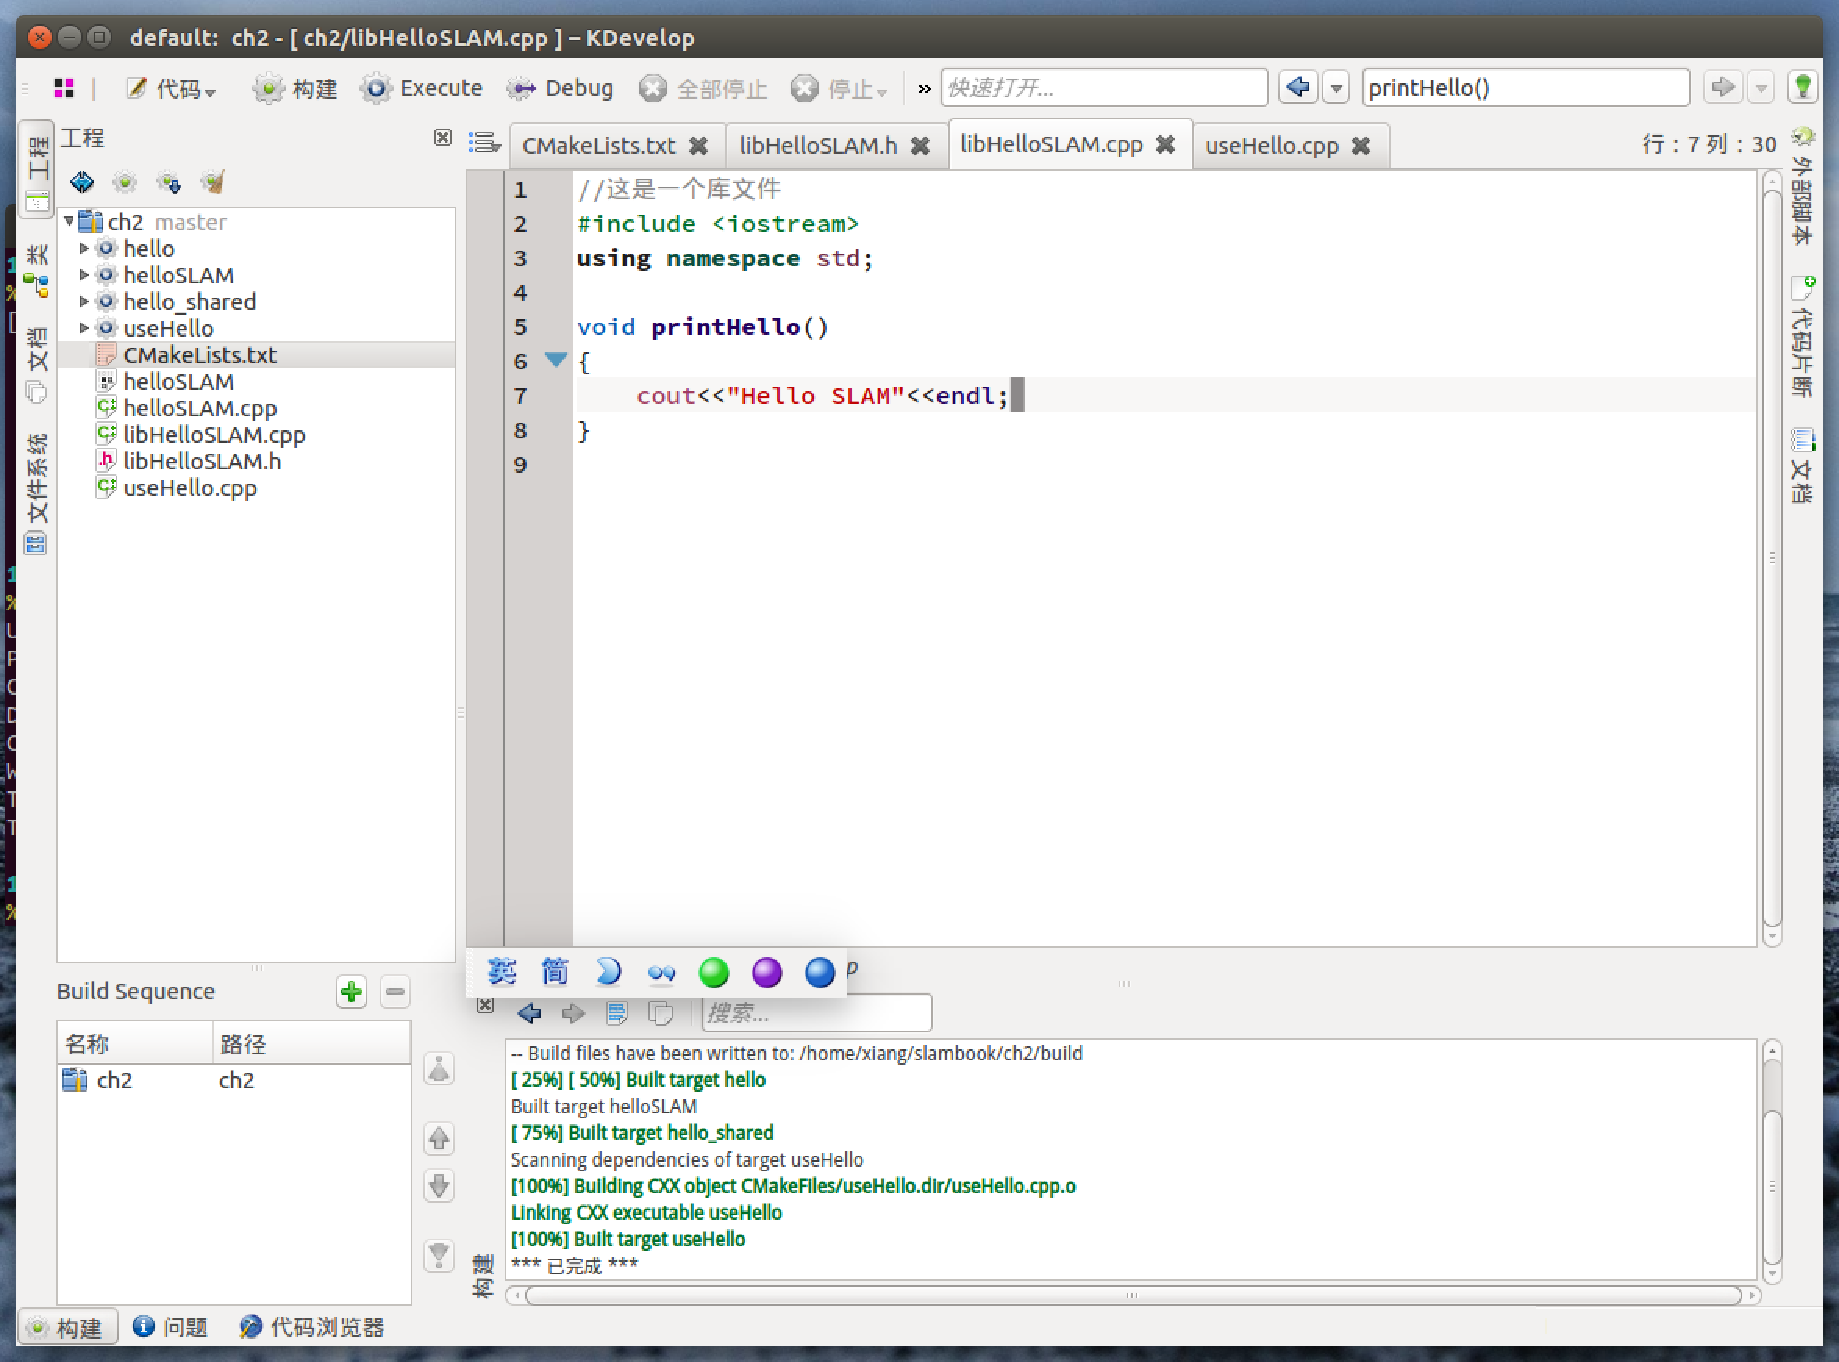
\includegraphics[width=0.8\textwidth]{whatIsSLAM/kdevelop.pdf}
	\caption{Kdevelop界面。}
	\label{fig:kdevelop}
\end{figure}

基本上,我们对一个IDE的功能要求它都具备,所以读者不妨尝试一下。有时候你会碰到一些问题,例如对某些模板类的解析响应比较缓慢等,确实它还不够完善。不过相比于其他IDE,它是不错的。

Kdevelop原生支持cmake工程。具体做法是,在终端建立CMakeLists.txt后,用Kdevelop中的“工程$\rightarrow$打开/导入工程”打开CMakeLists.txt。软件会询问你几个问题,并且默认建立一个build文件夹,帮你调用刚才的cmake和make命令。只要按下快捷键F8,这些都可以自动完成。\autoref{fig:kdevelop}的下面部分就显示了编译信息。

我们把适应IDE的任务交给读者自己来完成,而并不打算在书中进行详细说明。如果你是从Windows转过来的,会觉得它的界面与Visual C++或Visual Studio挺相似。请用Kdevelop打开刚才的工程然后进行编译,看看它输出什么信息。相信你会觉得比打开终端更方便一些。

不过,本节重点想讲的是如何在IDE中进行调试。在Windows下编程的同学多半会有在Visual Studio下断点调试的经历。不过在Linux中,默认的调试工具gdb只提供了文本界面,对新手来讲不太方便。有些IDE提供了断点调试功能(底层仍旧是gdb),Kdevelop就是其中之一。要使用Kdevelop的断点调试功能,你需要完成以下几件事:

\begin{enumerate}
	\item 在CMakeLists.txt中把工程调为Debug编译模式。
	\item 告诉Kdevelop你想运行哪个程序。如果有参数,也要配置它的参数和工作目录。
	\item 进入断点调试界面,就可以单步运行,看到中间变量的值了。
\end{enumerate}

\clearpage

第一步,在CMakeLists.txt中加入下面的命令来设置编译模式:
\begin{lstlisting}
set( CMAKE_BUILD_TYPE "Debug" )
\end{lstlisting}

cmake自带一些编译相关的内部变量,它们可以对编译过程进行更精细的控制。对于编译类型,通常有调试用的Debug模式与发布用的Release模式。在Debug模式中,程序运行较慢,但可以进行断点调试;而Release模式则速度较快,但没有调试信息。我们把程序设置成Debug模式,就能放置断点了。接下来,告诉Kdevelop你想启动哪个程序。

第二步,打开“运行$\rightarrow$配置启动器”,然后单击左侧的“Add New$\rightarrow$应用程序”。在这一步中,我们的任务是告诉Kdevelop想要启动哪一个程序。如\autoref{fig:launchConfigure}所示,既可以直接选择一个cmake的工程目标(也就是我们用add_executable指令构建的可执行程序),也可以直接指向一个二进制文件。建议使用第二种方式,根据我们的经验,这样更少出现问题。

\begin{figure}[!ht]
	\centering
	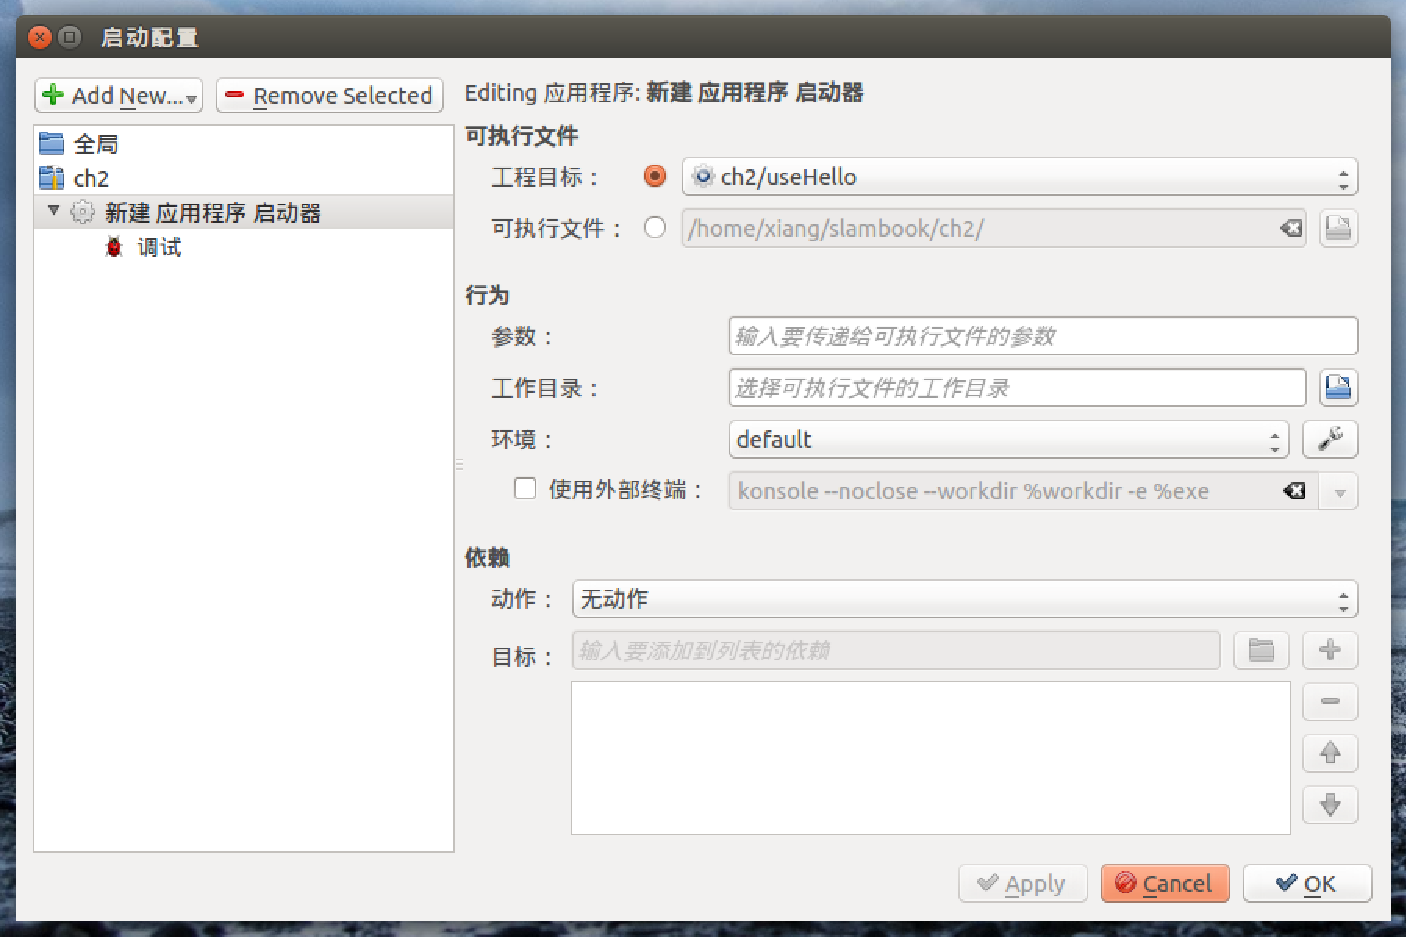
\includegraphics[width=0.8\textwidth]{whatIsSLAM/launchConfigure.pdf}
	\caption{启动器设置界面。}
	\label{fig:launchConfigure}
\end{figure}

在第二栏里,可以设置程序的运行参数和工作目录。有时程序是有运行参数的,它们会作为main函数的参数被传入。如果没有则可以留空,对于工作目录亦是如此。配置好这两项后,可以单击“OK”按钮保存配置结果。

刚才这几步我们配置了一个应用程序的启动项。对于每一个启动项,我们可以单击“Execute”按钮直接启动这个程序,也可单击“Debug”按钮对它进行断点调试。读者可以试着单击“Execute”按钮,查看输出的结果。现在,为了调试这个程序,单击printHello那行的左侧,增加一个断点。然后,单击“Debug”按钮,程序会停留在断点处等待,如\autoref{fig:debug}所示。

\begin{figure}[!htp]
	\centering
	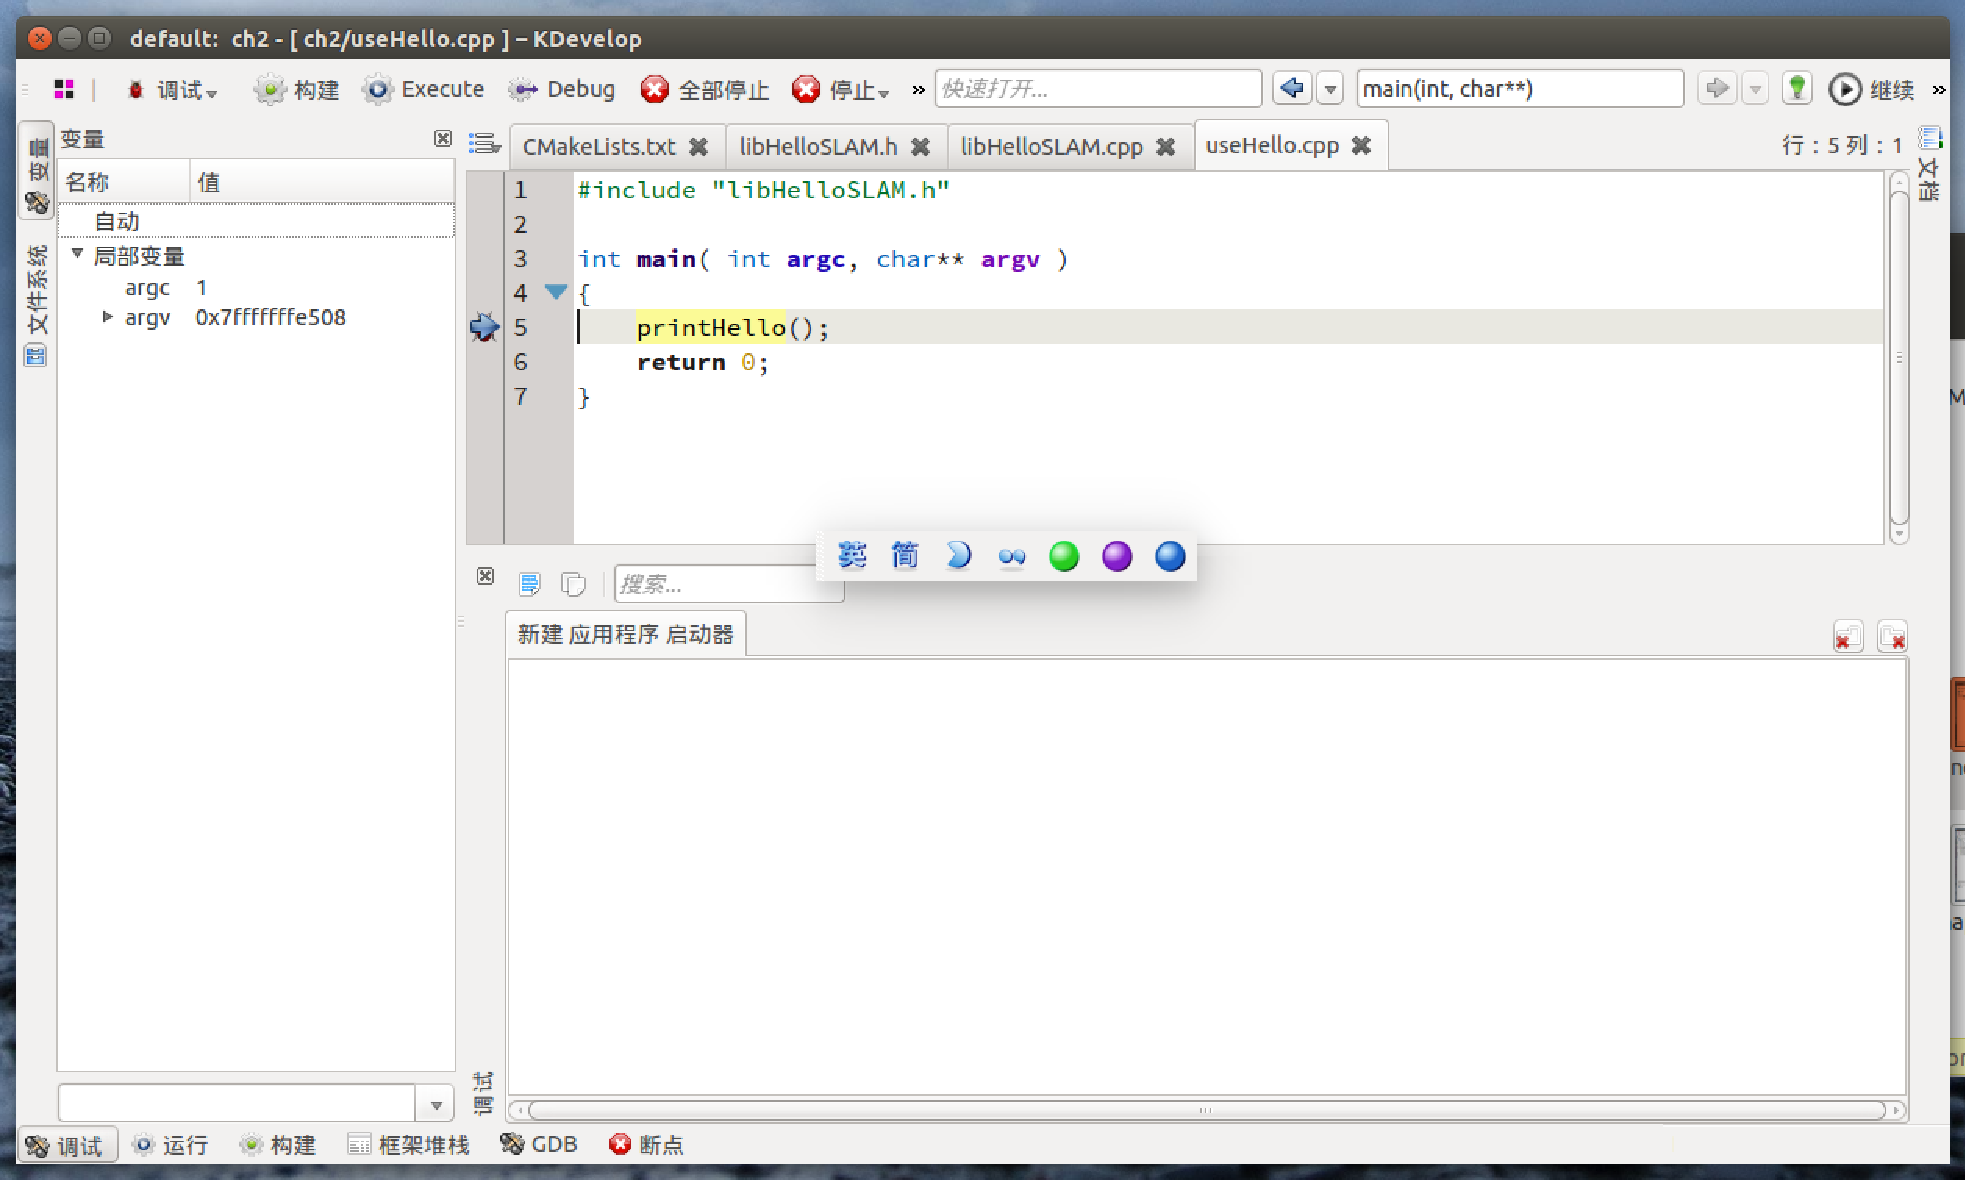
\includegraphics[width=0.8\textwidth]{whatIsSLAM/debug.pdf}
	\caption{调试界面。}
	\label{fig:debug}
\end{figure}

调试时,Kdevelop会切换到调试模式,界面会发生一点变化。在断点处,可以用单步运行(F10键)、单步跟进(F11键)、单步跳出(F12键)功能控制程序的运行。同时,可以点开左侧的界面,查看局部变量的值。或者选择“停止”按钮,结束调试。调试结束后,Kdevelop会回到正常的开发界面。

现在你应该熟悉了整个断点调试的流程。今后,如果在程序运行阶段发生了错误,导致程序崩溃,就可以用断点调试确定出错的位置,然后加以修正\footnote{而不是直接给我们发邮件询问怎么处理遇到的问题。}。%那么本讲也就到此为止了。你或许已经觉得我有些话唠了,所以在今后的实践部分中,我们不会再讲述如何新建build文件夹,调用cmake和make命令来编译程序了。我们相信读者应该掌握了这些简单的步骤。同样的,由于本书用到的大多第三方库都是cmake工程,所以你会不断熟悉这个编译过程,我们也就不再那么详细地解释了。

\section*{习题}
\begin{enumerate}
	\item 阅读文献\cite{Liu2016}和\cite{Liang2013},你能看懂其中的内容吗?
	\item[\optional] 阅读SLAM的综述文献,例如\cite{Cadena2016, Fuentes-Pacheco2015, Boal2014, Chen2012, Chen2007}等。这些文献关于SLAM的看法与本书有何异同?
	\item g++命令有哪些参数?怎么填写参数可以更改生成的程序文件名?
	\item 使用build文件夹来编译你的cmake工程,然后在Kdevelop中试试。
	\item 刻意在代码中添加一些语法错误,看看编译会生成什么样的信息。你能看懂g++的错误信息吗?
	\item 如果忘了把库链接到可执行程序上,编译会报错吗?报什么样的错?
	\item[\optional] 阅读《cmake实践》,了解cmake的其他语法。
	\clearpage
	\item[\optional] 完善hello SLAM小程序,把它做成一个小程序库,安装到本地硬盘中。然后,新建一个工程,使用find\_package找这个库并调用。
	\item[\optional] 寻找其他cmake教学材料,深入了解cmake,例如\url{https://github.com/TheErk/CMake-tutorial}。
	\item 找到Kdevelop的官方网站,看看它还有哪些特性。你都用上了吗?
	\item 如果在上一讲学习了Vim,请试试Kdevelop的Vim编辑功能。
\end{enumerate}